\chapter{\textit{Shift Graphs}}
\label{cap:shift}

\begin{definicao}
Um \textit{shift graph} de parâmetro $n$, denotado $S_n$, é um grafo cujos vértices são os pares ordenados $(a,b)$, onde $1 \leq a < b \leq n$, e dois vértices $(a,b)$ e $(c,d)$ são adjacentes se $b = c$ ou se $a = d$.
\end{definicao}

\begin{figure}[H]
\centering
\begin{tikzpicture}
    \node[anchor=south west,inner sep=0] at (0,0) {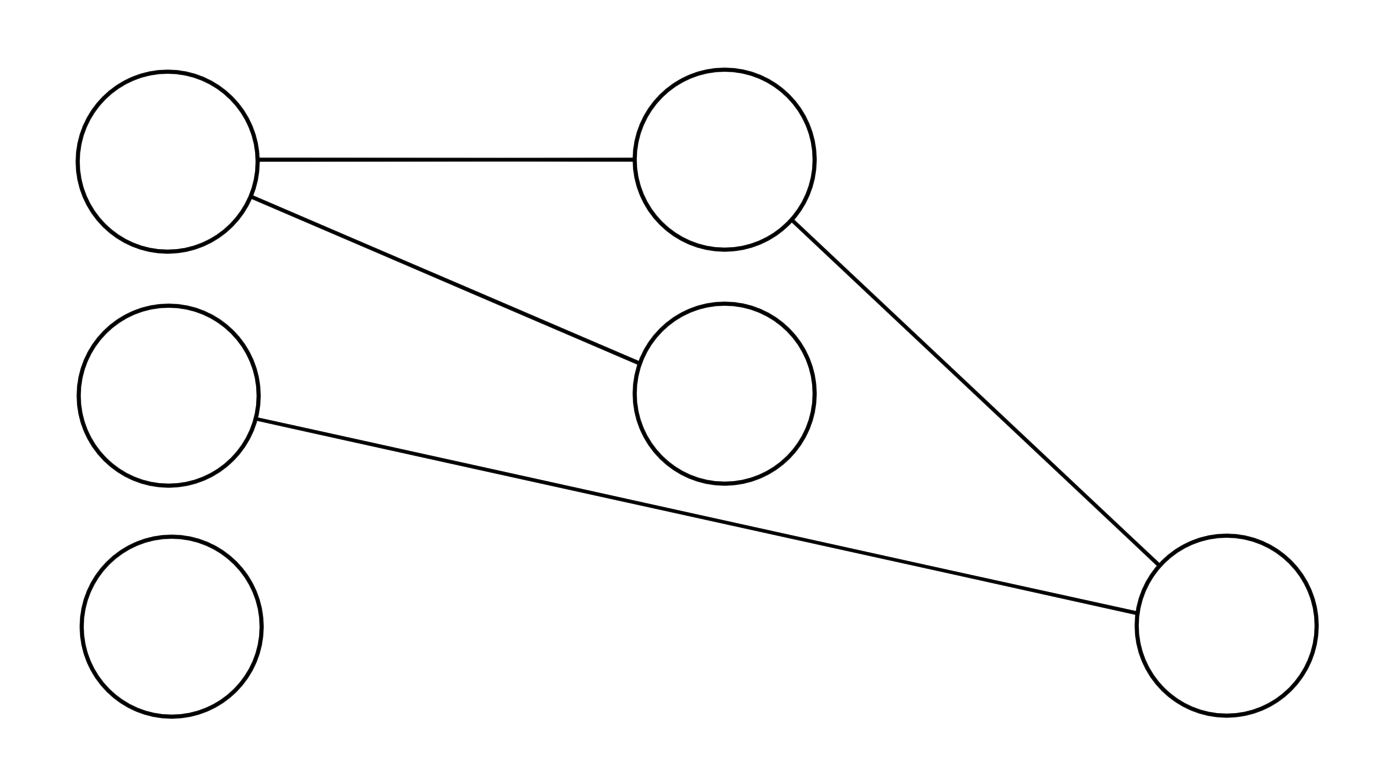
\includegraphics[width=0.5\textwidth]{figuras/ch_shift/shift-shift1.png}};
    \node at (1,3.6) {\large{$(1,2)$}};
    \node at (1,2.2) {\large{$(1,3)$}};
    \node at (1,0.8) {\large{$(1,4)$}};
    \node at (4.35,3.6) {\large{$(2,3)$}};
    \node at (4.35,2.2) {\large{$(2,4)$}};
    \node at (7.35,0.8) {\large{$(3,4)$}};
\end{tikzpicture}
\caption{O \textit{shift graph} $S_4$.}
\label{fig:shiftgraph}
\end{figure}

\begin{definicao}
Um \textit{shift graph} de parâmetro $n$ e ordem $r$, denotado $S_n^r$, é um grafo cujos vértices são as $(r+1)$-uplas $(a_0, a_1, a_2, \cdots, a_r)$, onde $1 \leq a_0 < a_1 < \cdots < a_r \leq n$, e dois vértices $a = (a_0, \cdots, a_r)$ e $b = (b_0, \cdots, b_r)$ são adjacentes se $a\setminus a_0 = b\setminus b_r$ ou $a\setminus a_r = b\setminus b_0$, ou seja, se os $r$ primeiros elementos de um vértice coincidem com os $r$ últimos elementos do outro vértice.
\end{definicao}

\begin{figure}[H]
\centering
\begin{tikzpicture}
    \node[anchor=south west,inner sep=0] at (0,0) {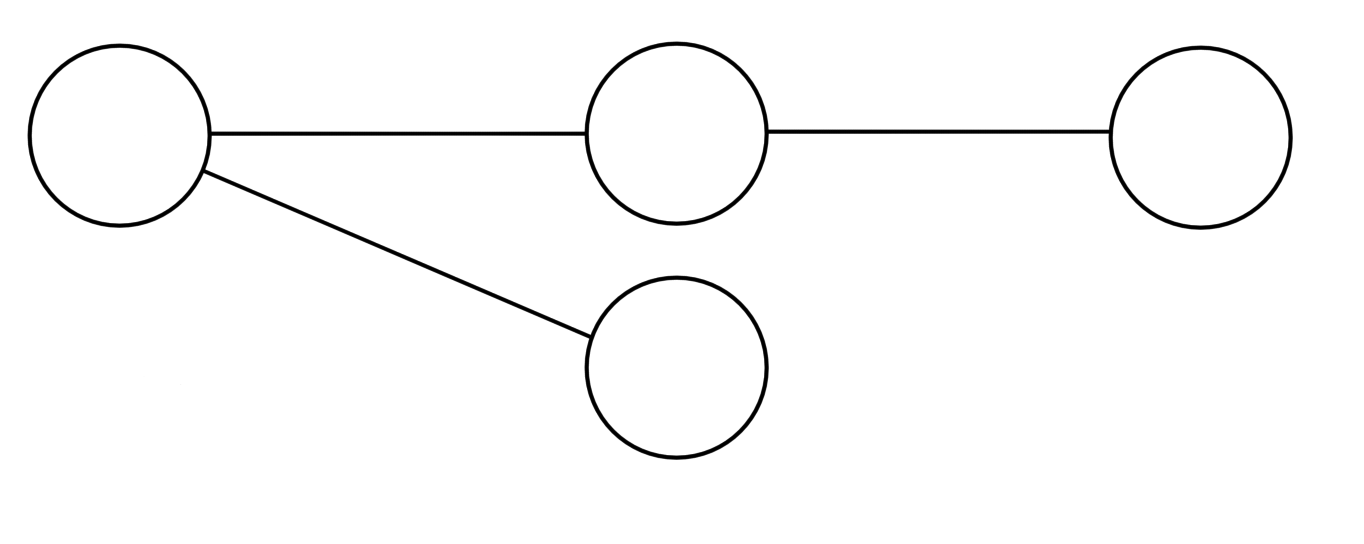
\includegraphics[width=0.6\textwidth]{figuras/ch_shift/shift-shiftorder2.png}};
    \node at (0.87,2.95) {$(1,2,3)$};
    \node at (4.9,2.95) {$(2,3,4)$};
    \node at (4.9,1.25) {$(2,3,5)$};
    \node at (8.7,2.95) {$(3,4,5)$};
\end{tikzpicture}
\caption{Alguns vértices de $S_5^{2}$.}
\label{fig:shiftgraphorder2}
\end{figure}

\begin{definicao}
Dado um grafo $G$, o grafo linha de $G$, denotado por $L(G)$, é o grafo definido da seguinte forma
\[V(L(G)) = \{e : e \in E(G)\}\]
\[E(L(G)) = \{vw : v,w \in E(G) \text{ e } |v \cap w| = 1\},\]
ou seja, os vértices do grafo $L(G)$ são as arestas de $G$, e dois vértices de $L(G)$ são adjacentes se as arestas correspondentes em $G$ têm um vértice em comum.

Ademais, o digrafo linha $L(D)$ de um digrafo $D$ é definido da seguinte forma
\[V(L(D)) = \{a : a \in A(D)\}\]
\[A(L(D)) = \{vw : v,w \in A(D) \text{ e } vw \text{ é um caminho dirigido em D}\},\]
ou seja, os vértices de $L(D)$ são os arcos de $D$, e $vw$ é um arco em $L(D)$ se existe um vértice $x$ em~$D$ tal que o arco $v$ entra em $x$, e o arco $w$ saia de $x$.
\end{definicao}

\begin{figure}[H]
\centering
\begin{tikzpicture}
    \node[anchor=south west,inner sep=0] at (0,0) {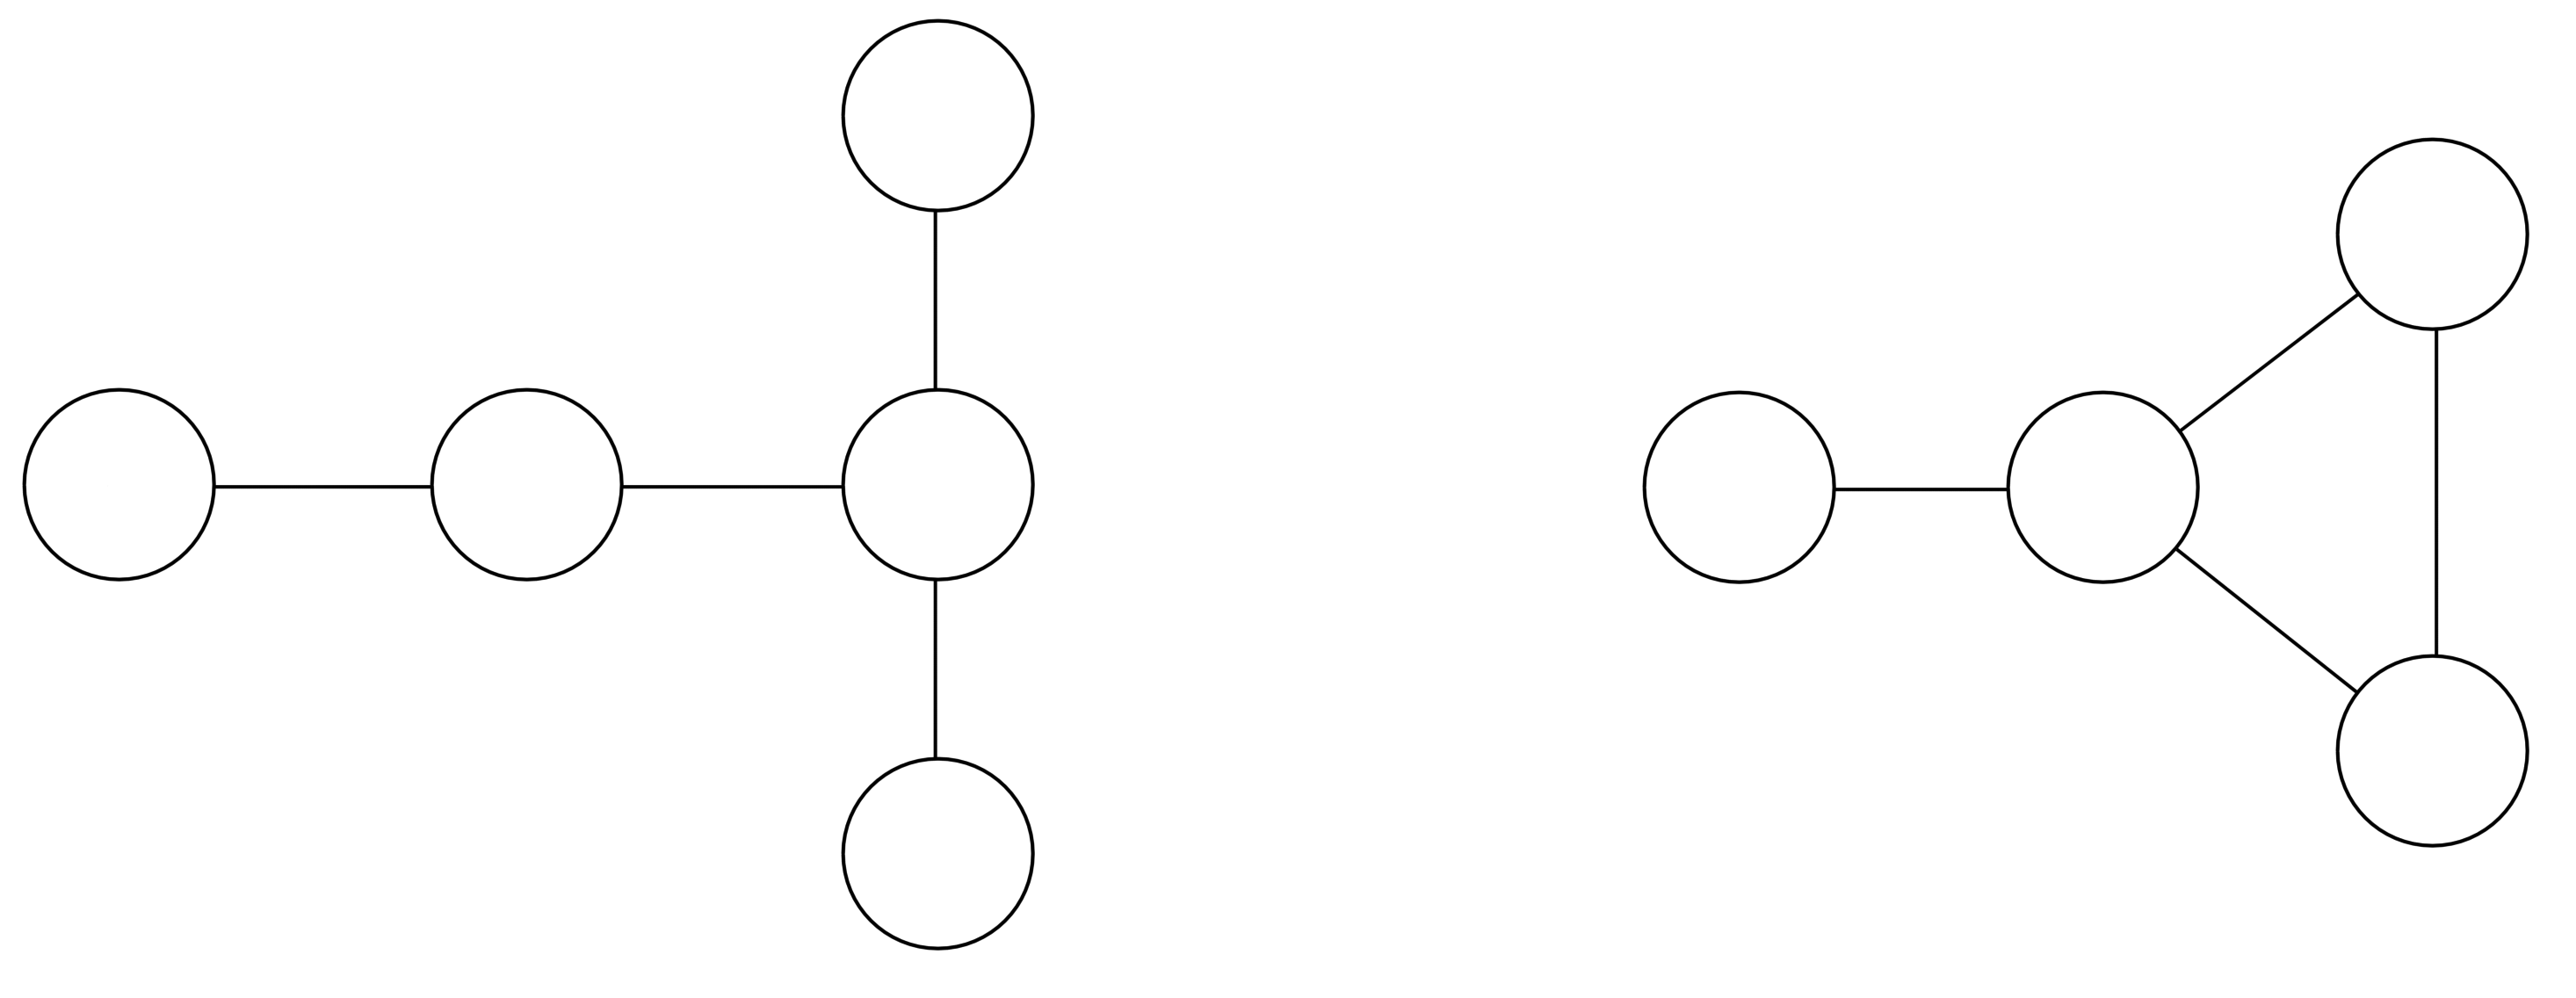
\includegraphics[width=0.85\textwidth]{figuras/ch_shift/shift-linegraph.png}};
    \node at (0.68,2.75) {\Large$v_1$};
    \node at (2.88,2.75) {\Large$v_2$};
    \node at (5.1,2.75) {\Large$v_3$};
    \node at (5.1,0.75) {\Large$v_4$};
    \node at (5.1,4.75) {\Large$v_5$};
    \node at (1.78,3.1) {\Large$e_1$};
    \node at (3.99,3.1) {\Large$e_2$};
    \node at (5.5,1.75) {\Large$e_3$};
    \node at (5.5,3.75) {\Large$e_4$};
    \node at (9.5,2.75) {\Large$e_1$};
    \node at (11.45,2.75) {\Large$e_2$};
    \node at (13.25,1.33) {\Large$e_3$};
    \node at (13.25,4.15) {\Large$e_4$};
\end{tikzpicture}
\caption{Um grafo $G$ (esquerda) e seu grafo linha $L(G)$ (direita).}
\label{fig:shiftlinegraph}
\end{figure}

\begin{figure}[H]
\centering
\begin{tikzpicture}
    \node[anchor=south west,inner sep=0] at (0.02,-0.07) {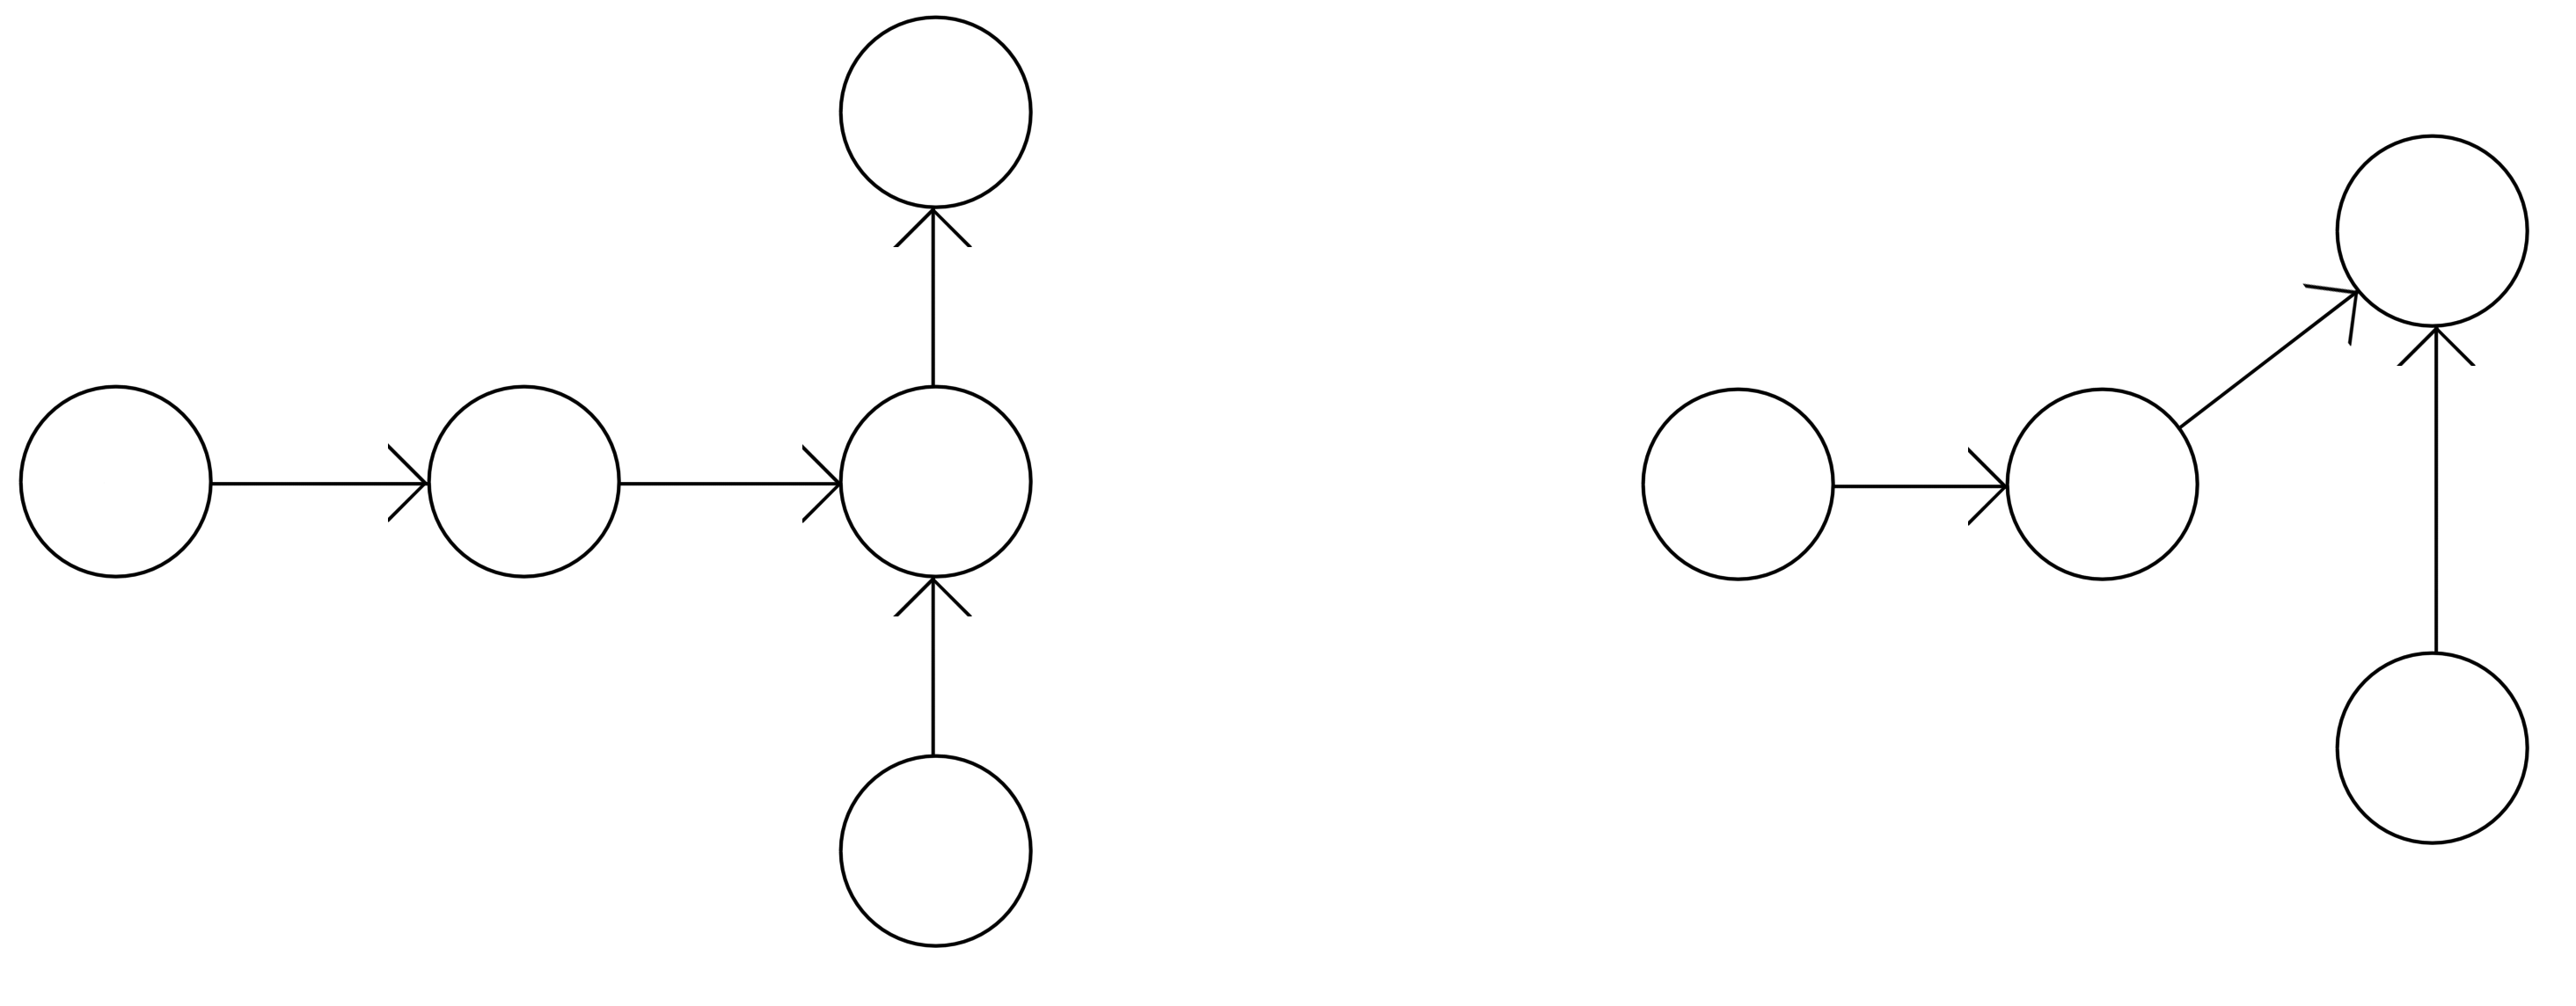
\includegraphics[width=0.85\textwidth]{figuras/ch_shift/shift-linedigraph.png}};
    \node at (0.68,2.75) {\Large$v_1$};
    \node at (2.88,2.75) {\Large$v_2$};
    \node at (5.1,2.75) {\Large$v_3$};
    \node at (5.1,0.75) {\Large$v_4$};
    \node at (5.1,4.75) {\Large$v_5$};
    \node at (1.78,3.1) {\Large$a_1$};
    \node at (3.99,3.1) {\Large$a_2$};
    \node at (5.5,1.75) {\Large$a_3$};
    \node at (5.5,3.75) {\Large$a_4$};
    \node at (9.5,2.75) {\Large$a_1$};
    \node at (11.45,2.75) {\Large$a_2$};
    \node at (13.25,1.33) {\Large$a_3$};
    \node at (13.25,4.15) {\Large$a_4$};
\end{tikzpicture}
\caption{Um digrafo $D$ (esquerda) e seu digrafo linha $L(D)$ (direita).}
\label{fig:shiftlinedigraph}
\end{figure}

Seja $L^1(G) := L(G)$, e para todo $r>1$ seja $L^r(G) := L(L^{r-1}(G))$. Denotamos $S_n^0 := K_n$ e~$L^0(G) := G$. 

Em busca de um contraexemplo para conjectura de Erd\H{o}s e Hajnal, Gábor Tardos pesquisou os \textit{shift graphs} de ordem $r$, porém concluindo que não são um contraexemplo. Portanto, temos o seguinte teorema.

\begin{teorema}\label{shiftteo}
A família dos \textit{shift graphs} de ordem $r$ respeita a conjectura de Erd\H{o}s e Hajnal. \cite{gabor2018cepa}
\end{teorema}

\section{Número Cromático}

\begin{afirmacao}\label{shiftchraff1}
O número cromático do \textit{shift graph} $S_n$ é $\ceil{\log_2(n)}$.
\end{afirmacao}

Para demonstrar a Afirmação \ref{shiftchraff1}, considere a seguinte afirmação.

\begin{afirmacao}\label{shiftafirm1}
Seja $D$ uma orientação transitiva de $K_n$. Então o \textit{shift graph} $S_n^r$ é uma simetrização de~$L^r(D)$.
\end{afirmacao}

\begin{proof}(Afirmação \ref{shiftafirm1})
Seja $V(D) = \{1,2,\cdots, n\}$, onde para cada $i < j$, existe um arco de $i$ para $j$. Mostraremos que a simetrização de $L(D)$ é isomorfa a $S_n^1$.

Denotemos por $(i,j)$ os arcos de $D$, onde $i < j$. Logo os vértices de $L(D)$ são os pares $(i,j)$ com~$i < j$. E para cada $1 \leq i < j < k \leq n$, existe em $D$ um arco de $i$ para $j$ e um arco de $j$ para~$k$. Logo em $L(D)$ existe um arco de $(i,j)$ para $(j,k)$. Temos então que

\[V(L(D)) = \{(i,j) : 1\leq i < j \leq n\},\]
\[A(L(D)) = \{(i,j)(j,k) : 1\leq i <j<k\leq n\}.\]

E temos que $S_n^1$ tem como conjunto de vértices os pares $(i,j)$ com $1\leq i<j\leq n$. E dois vértices~$(a,b)$ e $(c,d)$ são adjacentes se $a = d$ ou $b = c$. Logo temos que

\[V(S_n^1) = \{(i,j) : 1\leq i<j\leq n\},\]
\[E(S_n^1) = \{(i,j)(j,k) : 1\leq i<j<k\leq n\}.\]

Temos portanto que $L(D)$ e $S_n^1$ são ``quase isomorfos'', exceto pelo fato de que $L(D)$ é direcionado, portanto $S_n^1$ é uma simetrização de $L(D)$.

De forma semelhante, mostraremos que $S_n^r$ é uma simetrização de $L^r(D)$ para $r>1$.

Suponha que $S_n^{r-1}$ é uma simetrização de $L^{r-1}(D)$. Temos que $L^r(D) = L(L^{r-1}(D))$, e como temos que $L^{r-1}(D)$ é um direcionamento de $S_n^{r-1}$, sabemos que os vértices de $L^{r-1}(D)$ são as $r$-uplas $(v_0,\cdots,v_{r-1})$, onde $1\leq v_0 < \cdots < v_{r-1} \leq n$, e para cada escolha de~$1\leq v_0 < \cdots < v_{r} \leq n$, existe um arco de $(v_0,\cdots,v_{r-1})$ para $(v_1,\cdots,v_r)$.

Para cada sequência $1\leq v_0 < \cdots < v_{r} \leq n$, denote por $(v_0,\cdots,v_{r})$ o arco de $(v_0,\cdots,v_{r-1})$ para $(v_1,\cdots,v_r)$ em $L^{r-1}(D)$. Logo $L(L^{r-1}(D))$ tem como vértices as $(r+1)$-uplas $(v_0,\cdots,v_{r})$, onde $1\leq v_0 < \cdots < v_r \leq n$.

Temos que para cada $1\leq v_0 < \cdots < v_{r+1} \leq n$, existe em $L^{r-1}(D)$ um arco de $(v_0,\cdots,v_{r-1})$ para $(v_1,\cdots,v_r)$ e um arco de $(v_1,\cdots,v_{r})$ para $(v_2,\cdots,v_{r+1})$. Portanto em $L(L^{r-1}(D))$, para cada~$1\leq v_0 < \cdots < v_{r+1} \leq n$ existe um arco de $(v_0,\cdots,v_{r})$ para $(v_1,\cdots,v_{r+1})$. Logo

\[V(L^r(D)) = \{(v_0,\cdots,v_{r}) : 1\leq v_0 < \cdots < v_r \leq n\},\]
\[A(L^r(D)) = \{(v_0,\cdots,v_{r})(v_1,\cdots,v_{r+1}) : 1\leq v_0 < \cdots < v_{r+1} \leq n\}.\]

E os vértices de $S_n^r$ são as $(r+1)$-uplas $(v_0, v_1, \cdots, v_r)$, onde $1\leq v_0 < v_1 < \cdots < v_r \leq n$. E para cada $1 \leq v_0 < v_1 <\cdots < v_r < v_{r+1} \leq n$, os vértices $(v_0, \cdots, v_r)$ e $(v_1, \cdots, v_{r+1})$ são adjacentes. Então 

\[V(S_n^r) = \{(v_0, v_1, \cdots, v_r) : 1 \leq v_0 < \cdots < v_r \leq n\},\]
\[E(S_n^r) = \{(v_0, v_1, \cdots, v_r)(v_1, v_2, \cdots, v_{r+1}) : 1 \leq v_0 < \cdots < v_{r+1} \leq n\}.\]

Temos portanto que $S_n^r$ é uma simetrização de $L^r(D)$.
\end{proof}

Podemos então demonstrar que o número cromático de $S_n$ é $\ceil{\log_2(n)}$.

\begin{proof}(Afirmação \ref{shiftchraff1})
Seja $D$ uma orientação transitiva de $K_n$. Temos que $S_n$ é uma simetrização de $L(D)$. 

Para mostrar que $\chi(S_n) \geq \ceil{\log_2(n)}$, suponha que $S_n$ pode ser colorido com~$\ceil{\log_2(n)} - 1$ cores e tome uma $(\ceil{\log_2(n)} -1)$-coloração de $S_n$. Tal coloração dos vértices de~$S_n$ corresponde a uma $(\ceil{\log_2(n)}-1)$-coloração dos arcos de $D$. Para cada vértice de $D$ atribua um vetor binário tal que cada entrada corresponda a uma das $\ceil{\log_2(n)}-1$ cores dos arcos, e cada entrada tem valor $1$ se algum arco da cor correspondente chega no vértice, e $0$ caso contrário. 

\begin{figure}[H]
\centering
%\resizebox{2cm}{!}{
\begin{tikzpicture}
    \node[circle, draw=black] (A) at (0,0) {$v$};
    
    \draw[->] (-1.5,-1) to node[midway, below] {$i$} (A);
    \draw[->] (-1.5,1) to node[midway, above] {$j$} (A);
    
    \node[right = of A] (B) {cor$(v) = \{\cdots,1,\cdots,1,\cdots\}$};
    \node[above left = 0.1 and -2.9 of B] (C) {$i$};
    \node[right = 0.7 of C] (D) {$j$};
\end{tikzpicture}
%}
\caption{Arcos de cor $i$ e $j$ chegam em $v$, logo a cor de $v$ contém $1$ nas posições $i$ e $j$.}
\label{fig:shiftchromaticvector}
\end{figure}

Temos que tal coloração é própria, pois caso exista um arco $vw$ monocromático em $D$, temos que existe um arco que chega em $v$ com a mesma cor do arco entre $v$ e $w$, o que não é possível, pois tal configuração é um arco monocromático em $L(D)$. 

E temos que tal coloração usa $2^{(\ceil{\log_2(n)}-1)} < n$ cores, contradição, pois $D$ é um digrafo completo, e logo precisa de $n$ cores.

E para mostrar que $\chi(S_n) \leq \ceil{\log_2(n)}$, considere a seguinte coloração de $D$.

Sejam $v_1, v_2,\cdots, v_n$ os vértices de $D$ em ordem topológica. E sejam $A_1, \cdots, A_m$ os subconjuntos de $[\ceil{\log_2(n)}]$ em ordem não-crescente de tamanho, ou seja, se $i > j$, então $|A_i| \leq |A_j|$.

Para cada vértice $v_i$, atribua o conjunto $A_i$. Colorimos cada arco $v_iv_j$ de $D$ com um elemento de $A_i\setminus A_j$. Note que é sempre possível escolher um tal elemento, pois caso $|A_i| > |A_j|$, claramente existe algum elemento de $A_i$ que não pertence a $A_j$, e caso $|A_i| = |A_j|$, temos que $A_i \neq A_j$, e logo existe algum elemento em $A_i\setminus A_j$.

\begin{figure}[H]
\centering
%\resizebox{2cm}{!}{
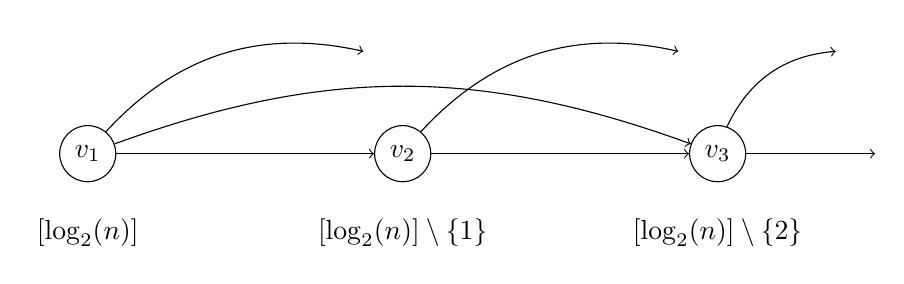
\begin{tikzpicture}
    \node[circle, draw=black] (A) at (0,0) {$v_1$};
    \node[circle, draw=black] (B) at (4,0) {$v_2$};
    \node[circle, draw=black] (C) at (8,0) {$v_3$};
    
    \draw[->] (A) to [bend left=20] (C);
    \draw[->] (A) to (B);
    \draw[->] (B) to (C);
    \draw[->] (C) to (10,0);
    \draw[->] (C) to [bend left=30] (9.5,1.3);
    \draw[->] (B) to [bend left=30] (7.5,1.3);
    \draw[->] (A) to [bend left=30] (3.5,1.3);
    
    \node at (0,-1) {$[\ceil{\log_2(n)}]$};
    \node at (4,-1) {$[\ceil{\log_2(n)}]\setminus \{1\}$};
    \node at (8,-1) {$[\ceil{\log_2(n)}]\setminus \{2\}$};
\end{tikzpicture}
%}
\caption{Cada vértice de $D$ é colorido com um subconjunto distinto de $[\ceil{\log_2(n)}]$, atribuídos em ordem não-crescente de tamanho segundo a ordem dos vértices de $D$.}
\label{fig:shiftchromaticsetcoloring}
\end{figure}

Note que em nenhum vértice entram e saem arcos de uma mesma cor, pois todo arco que entra em um vértice $v_i$ não pertence ao conjunto $A_i$, e todo arco que sai de $v_i$ pertence ao conjunto $A_i$.

A atribuição anterior corresponde a uma $\ceil{\log_2(n)}$-coloração própria dos vértices de $L(D)$. E logo corresponde a uma $\ceil{\log_2(n)}$-coloração própria dos vértices de $S_n$.

Portanto, concluímos que $\chi(S_n) = \ceil{\log_2(n)}$.
\end{proof}

De forma geral, o número cromático de $S_n^r$ é~$(1+o(1))\log_2 \log_2 \cdots \log_2 (n)$, onde o logaritmo é tomado $r$ vezes \cite{erdos1968chromatic}.

%%%%%%%%%%%%%%%%%%%%%%%%%%%%%%%%%%%%%%%%%%%%%%%%%%%%%%%%%%%%%%%%%%%%%%%%%%%%%
% ^ Escrever onde quer chegar com isso
%%%%

\section{Esboço da prova}

A seguir, um esboço da demonstração de que os \textit{shift graphs} respeitam a conjectura de Erd\H{o}s e Hajnal. Usando o Lema Local de Lovász, mostraremos que existe um subgrafo $H$ de $S_n^r$ tal que $H$ tem cintura grande e contém pelo menos uma aresta de cada $K_{d,d}$ de $S_n^r$, onde $d$ é $o(n)$.

%Seja $D$ uma orientação transitiva de $K_n$. Temos que $L^r(D)$ é isomorfo a um direcionamento de $S_n^r$, e usando o lema local de Lovász, encontraremos um subgrafo $H$ de $S_n^r$ tal que $H$ tem cintura grande e contém pelo menos uma aresta de cada $K_{d,d}$ de $S_n^r$, onde $d$ é $o(n)$.

Queremos mostrar que o número cromático de $H$ não é limitado por uma constante, ou seja, que $\chi(H) \rightarrow \infty$ conforme $n \rightarrow \infty$.

Mostraremos que se temos uma $t$-coloração de $S_n^r$ sem $K_{d,d}$ monocromático, existe uma $2^t$-coloração de $S_n^{r-1}$ sem $K_{td,td}$ monocromático. E logo existe uma $t'$-coloração de $S_n^i$ sem $K_{d',d'}$ monocromático para cada $i\in [0,r]$, para algum par de inteiros $t'$ e $d'$.

Uma coloração própria de $H$ é uma coloração de $S_n^r$ sem $K_{d,d}$ monocromático. Então se $H$ tem número cromático limitado por constante, então em particular, existem constantes $t'$ e $d'$ tais que~$S_n^0$ pode ser colorido com $t'$ cores sem $K_{d',d'}$ monocromático para todo $n$.

Mas como $S_n^0$ é isomorfo ao $K_n$, então temos constantes $t'$ e $d'$ tais que existe uma $t'$-coloração de~$K_n$ sem $K_{d',d'}$ monocromático para todo $n$. Contradição, pois note que um conjunto de $2d'$ vértices coloridos com uma mesma cor é um $K_{d',d'}$ monocromático, e com apenas $t' < \infty$ cores, alguma cor ocorre pelo menos $2d'$ vezes. Logo o número cromático de $H$ não é limitado por uma constante.

%Uma coloração própria de $H$ é uma coloração de $S_n^r$ sem $K_{d,d}$ monocromático. Então suponha que o número cromático de $H$ é limitado por uma constante, existem constantes $t'$ e $d'$ tais que $S_n^i$ pode ser $t'$-colorido sem $K_{d',d'}$ monocromático, em particular, existe tal coloração para $S_n^0 = D$. Contradição, pois note que um conjunto de $2d'$ vértices coloridos com uma mesma cor é um $K_{d',d'}$ monocromático em $D$, e com apenas $t' < \infty$ cores, alguma cor ocorre pelo menos $2d'$ vezes em $D$ conforme $n\rightarrow\infty$. Logo o número cromático de $H$ não é limitado por uma contante.

\section{Prova do Teorema}

% \begin{afirmacao}\label{shiftafirm1}
% Seja $D$ uma orientação transitiva de $K_n$. Então o \textit{shift graph} $S_n^r$ é uma simetrização de~$L^r(D)$.
% \end{afirmacao}

% \begin{proof}(Afirmação \ref{shiftafirm1})
% Seja $V(D) = \{1,2,\cdots, n\}$, onde para cada $i < j$, existe um arco de $i$ para $j$. Mostraremos que a simetrização de $L(D)$ é isomorfa a $S_n^1$.

% Denotemos por $(i,j)$ os arcos de $D$, onde $i < j$. Logo os vértices de $L(D)$ são os pares $(i,j)$ com~$i < j$. E para cada $1 \leq i < j < k \leq n$, existe em $D$ um arco de $i$ para $j$ e um arco de $j$ para~$k$. Logo em $L(D)$ existe um arco de $(i,j)$ para $(j,k)$. Temos então que

% \[V(L(D)) = \{(i,j) : 1\leq i < j \leq n\},\]
% \[A(L(D)) = \{(i,j)(j,k) : 1\leq i <j<k\leq n\}.\]

% E temos que $S_n^1$ tem como conjunto de vértices os pares $(i,j)$ com $1\leq i<j\leq n$. E dois vértices~$(a,b)$ e $(c,d)$ são adjacentes se $a = d$ ou $b = c$. Logo temos que

% \[V(S_n^1) = \{(i,j) : 1\leq i<j\leq n\},\]
% \[E(S_n^1) = \{(i,j)(j,k) : 1\leq i<j<k\leq n\}.\]

% Temos portanto que $L(D)$ e $S_n^1$ são ``quase isomorfos'', exceto pelo fato de que $L(D)$ é direcionado, portanto $S_n^1$ é uma simetrização de $L(D)$.

% %%Denotemos por $(i,j)$ os arcos de $D$, onde $i < j$. Então os vértices de $L(D)$ são os pares $(i,j), i<j$. E os vértices de $S_n^1$ são os pares $(i,j), 1\leq i < j \leq n$. Claramente existe uma bijeção entre os vértices de $L(D)$ e os vértices de $S_n^1$.

% %%Para cada $1\leq i < j < k \leq n$, existe em $D$ um arco de $i$ para $j$ e um arco de $j$ para $k$, logo em $L(D)$ existe um arco de $(i,j)$ para $(j,k)$. E em $S_n^1$, para cada $1\leq i < j < k \leq n$ existe uma aresta entre $(i,j)$ e $(j,k)$. Claramente existe uma bijeção entre os arcos de $L(D)$ e as arestas de $S_n^1$. Temos portanto que $L(D)$ e $S_n^1$ são ``quase isomorfos'', exceto pelo fato de que $L(D)$ é direcionado, portanto $S_n^1$ é uma simetrização de $L(D)$.

% De forma semelhante, mostraremos que $S_n^r$ é uma simetrização de $L^r(D)$ para $r>1$.

% Temos que $L^r(D) = L(L^{r-1}(D))$, e como $L^{r-1}(D)$ é um direcionamento de $S_n^{r-1}$, sabemos que os vértices de $L^{r-1}(D)$ são as $r$-uplas $(v_0,\cdots,v_{r-1})$, onde $1\leq v_0 < \cdots < v_{r-1} \leq n$, e temos que para cada escolha de $1\leq v_0 < \cdots < v_{r} \leq n$, existe um arco de $(v_0,\cdots,v_{r-1})$ para $(v_1,\cdots,v_r)$.

% Para cada sequência $1\leq v_0 < \cdots < v_{r} \leq n$, denote por $(v_0,\cdots,v_{r})$ o arco de $(v_0,\cdots,v_{r-1})$ para $(v_1,\cdots,v_r)$ em $L^{r-1}(D)$. Logo $L(L^{r-1}(D))$ tem como vértices as $(r+1)$-uplas $(v_0,\cdots,v_{r})$, onde $1\leq v_0 < \cdots < v_r \leq n$.

% Temos que para cada $1\leq v_0 < \cdots < v_{r+1} \leq n$, existe em $L^{r-1}(D)$ um arco de $(v_0,\cdots,v_{r-1})$ para $(v_1,\cdots,v_r)$ e um arco de $(v_1,\cdots,v_{r})$ para $(v_2,\cdots,v_{r+1})$. Logo em $L(L^{r-1}(D))$, para cada $1\leq v_0 < \cdots < v_{r+1} \leq n$ existe um arco de $(v_0,\cdots,v_{r})$ para $(v_1,\cdots,v_{r+1})$. Logo

% \[V(L^r(D)) = \{(v_0,\cdots,v_{r}) : 1\leq v_0 < \cdots < v_r \leq n\},\]
% \[A(L^r(D)) = \{(v_0,\cdots,v_{r})(v_1,\cdots,v_{r+1}) : 1\leq v_0 < \cdots < v_{r+1} \leq n\}.\]

% E os vértices de $S_n^r$ são as $(r+1)$-uplas $(v_0, v_1, \cdots, v_r)$, onde $1\leq v_0 < v_1 < \cdots < v_r \leq n$. E para cada $1 \leq v_0 < v_1 <\cdots < v_r < v_{r+1} \leq n$, os vértices $(v_0, \cdots, v_r)$ e $(v_1, \cdots, v_{r+1})$ são adjacentes. Então 

% \[V(S_n^r) = \{(v_0, v_1, \cdots, v_r) : 1 \leq v_0 < \cdots < v_r \leq n\},\]
% \[E(S_n^r) = \{(v_0, v_1, \cdots, v_r)(v_1, v_2, \cdots, v_{r+1}) : 1 \leq v_0 < \cdots < v_{r+1} \leq n\}.\]

% %%Temos que $L^r(D) = L(L^{r-1}(D))$, e como $L^{r-1}(D)$ é um direcionamento de $S_n^{r-1}$, sabemos que os vértices de $L^{r-1}(D)$ são as $r$-uplas $(v_0,\cdots,v_{r-1})$, onde $1\leq v_0 < \cdots < v_{r-1} \leq n$, e temos que para cada escolha de $1\leq v_0 < \cdots < v_{r} \leq n$, existe um arco de $(v_0,\cdots,v_{r-1})$ para $(v_1,\cdots,v_r)$.

% %%Então para cada $1\leq v_0 < \cdots < v_{r} \leq n$, denote por $(v_0,\cdots,v_{r})$ o arco de $(v_0,\cdots,v_{r-1})$ para $(v_1,\cdots,v_r)$ em $L^{r-1}(D)$. Portanto temos uma bijeção entre os vértices de $L(L^{r-1}(D))$ e os vértices de $S_n^r$.

% %%E para cada $1\leq v_0 < \cdots < v_{r+1} \leq n$, existe em $L^{r-1}(D)$ um arco de $(v_0,\cdots,v_{r-1})$ para $(v_1,\cdots,v_r)$ e um arco de $(v_1,\cdots,v_{r})$ para $(v_2,\cdots,v_{r+1})$. Logo em $L(L^{r-1}(D))$, para cada $1\leq v_0 < \cdots < v_{r+1} \leq n$ existe um arco de $(v_0,\cdots,v_{r})$ para $(v_1,\cdots,v_{r+1})$.

% Temos portanto que $S_n^r$ é uma simetrização de $L^r(D)$.
% \end{proof}

\begin{lema}\label{shiftlema1}
Seja $D$ um grafo dirigido. Se $L(D)$ pode ser colorido com $t$ cores sem $K_{d,d}$ monocromático, então $D$ pode ser colorido com $2^t$ cores sem $K_{td,td}$ monocromático.
\end{lema}

\begin{proof}{(Lema \ref{shiftlema1})}
Considere uma $t$-coloração de $L(D)$ sem $K_{d,d}$ monocromático. Tal coloração corresponde a uma coloração dos arcos de $D$ com $t$ cores.

Considere a seguinte coloração dos vértices de $D$. Cada vértice é colorido com um vetor binário de $t$ entradas, correspondentes às $t$ cores dos arcos, onde cada entrada é $1$ caso entrem pelo menos~$d$ arcos da cor correspondente, e $0$ caso contrário.

\begin{figure}[H]
\centering
\begin{tikzpicture}
    \node[anchor=south west,inner sep=0] at (0.02,-0.07) {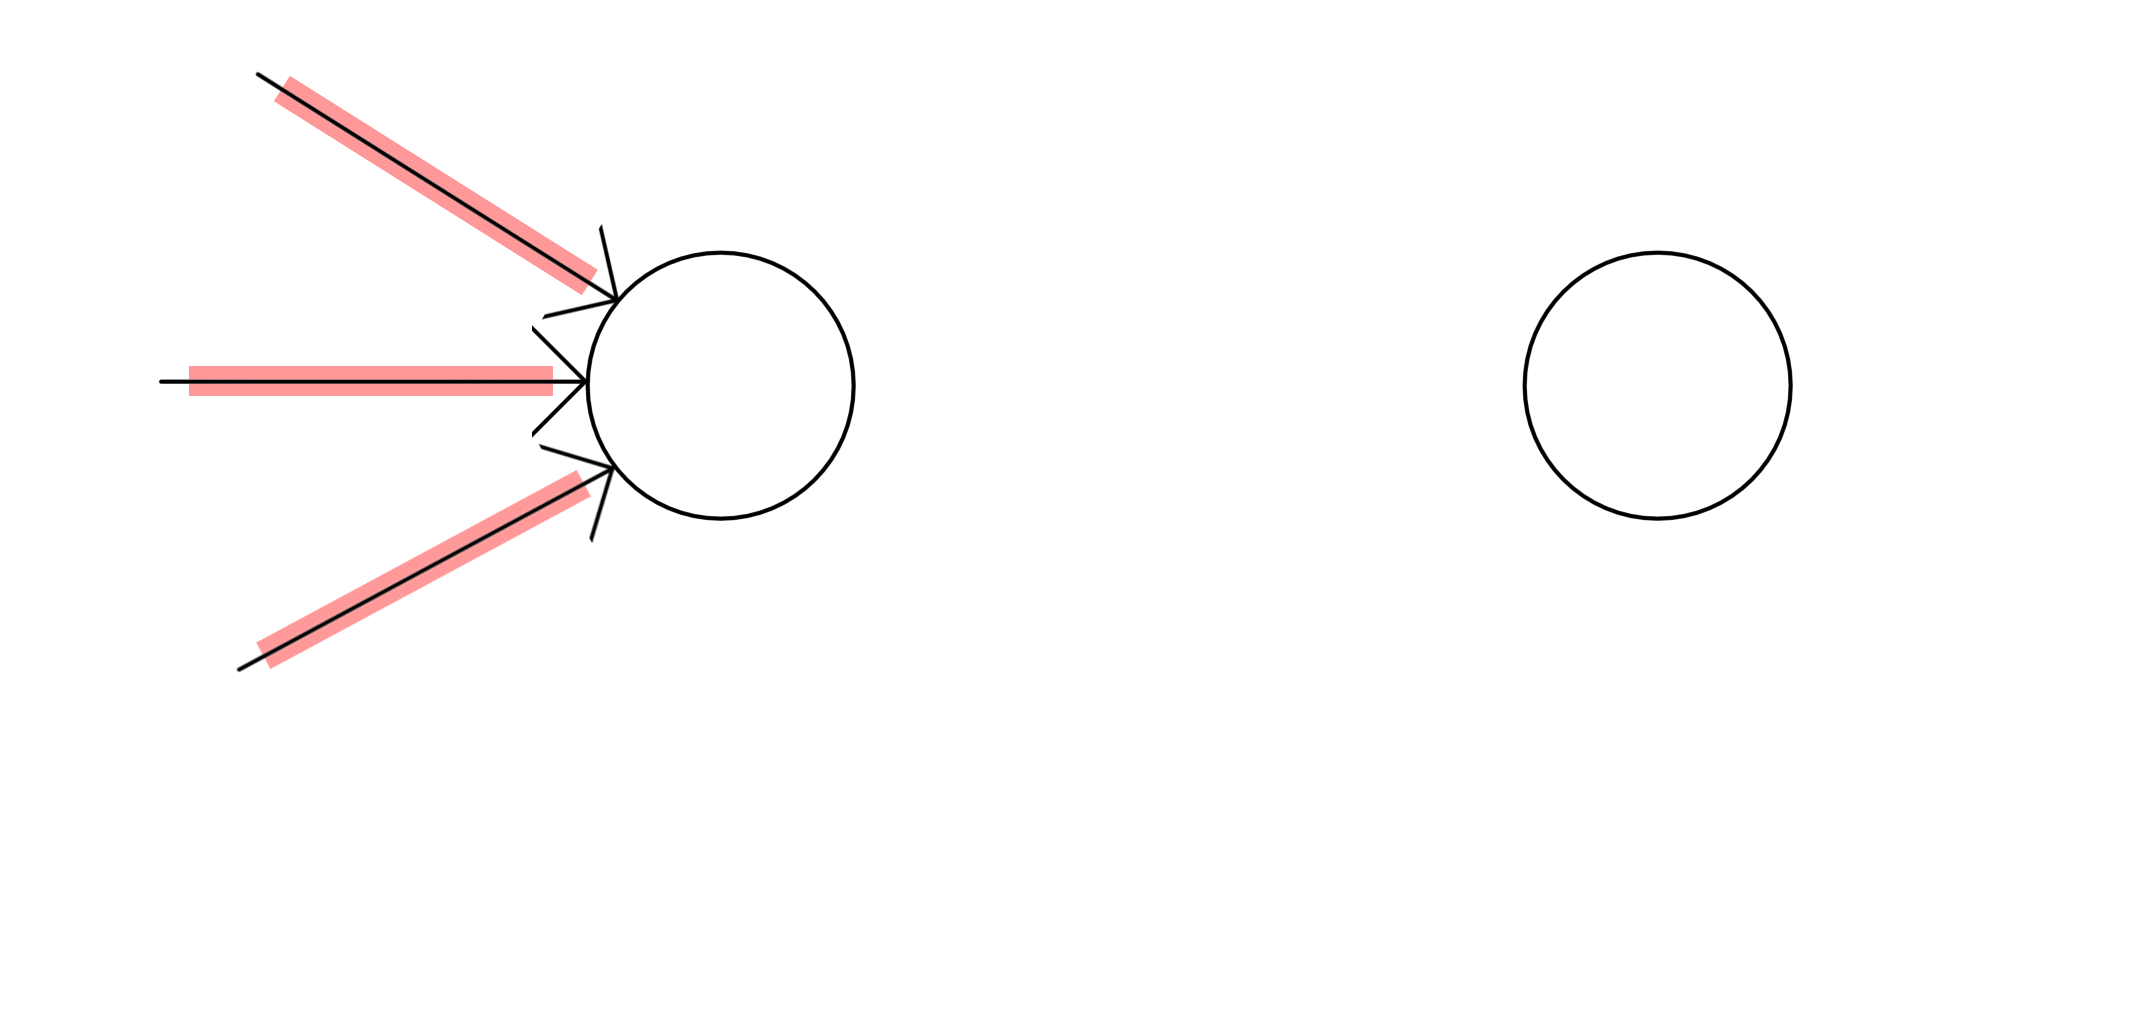
\includegraphics[width=0.85\textwidth]{figuras/ch_shift/shift-arccoloringtovertex.png}};
    \node at (10.85,1.6) {\large$(\cdots, 1, \cdots)$};
    \node at (10.85,1.0) {\large$i$};
    \draw [decorate,decoration={brace,amplitude=10pt},xshift=0pt,yshift=0pt](4.0,1.6) -- (0.8,1.6) node [black,midway,yshift=-0.6cm] {$\geq d$ arcos de cor $i$.};
\end{tikzpicture}
\caption{A $i$-ésima entrada da cor de um vértice é $1$ se nele entram pelo menos $d$ arcos de cor $i$.}
\label{fig:shiftarccoloringtovertex}
\end{figure}

Mostraremos que esta coloração é tal como descrita pelo lema. 

Claramente, temos no máximo $2^t$ cores. Então basta mostrar que tal coloração não contém $K_{td,td}$ monocromático.

Suponha por contradição que existe $K_{td,td}$ monocromático de cor $v$, e digamos que os arcos vão do conjunto de vértices $A$ para o conjunto de vértices $B$. Seja $k$ o número de entradas $0$ em $v$. Para cada vértice de $B$, sabemos que chegam no máximo $d-1$ arcos com cada uma das $k$ cores de entrada $0$ em $v$, pois caso contrário tal cor não teria entrada $0$ em $v$. Logo, no máximo $ktd(d-1)$ arcos do $K_{td,td}$ tem uma das $k$ cores de entrada $0$. Portanto, temos pelo menos $t^2d^2 - ktd(d-1) = td(td - k(d-1))$ arcos com uma das $t-k$ cores de entrada $1$ em $v$.

Como temos $|A| = td$ e $td(td - k(d-1))$ arcos com uma das cores de entrada $1$, pelo princípio da casa dos pombos, de algum vértice de $A$ saem pelo menos $td - k(d-1) = d(t-k) + k$ arcos com uma das cores de entrada $1$. E como temos $t-k$ cores com entrada $1$, alguma delas ocorre pelo menos $d + k/(t-k)$ vezes.

Temos portanto que de algum vértice de $A$ saem pelo menos $d$ arcos com uma cor de entrada~$1$, e entram pelo menos $d$ arcos da mesma cor (pois tal cor tem entrada $1$ em $v$). Tal configuração corresponde a um $K_{d,d}$ monocromático em $L(D)$, contradição.

\begin{figure}[H]
\centering
\begin{tikzpicture}
    \node[anchor=south west,inner sep=0] at (0,0) {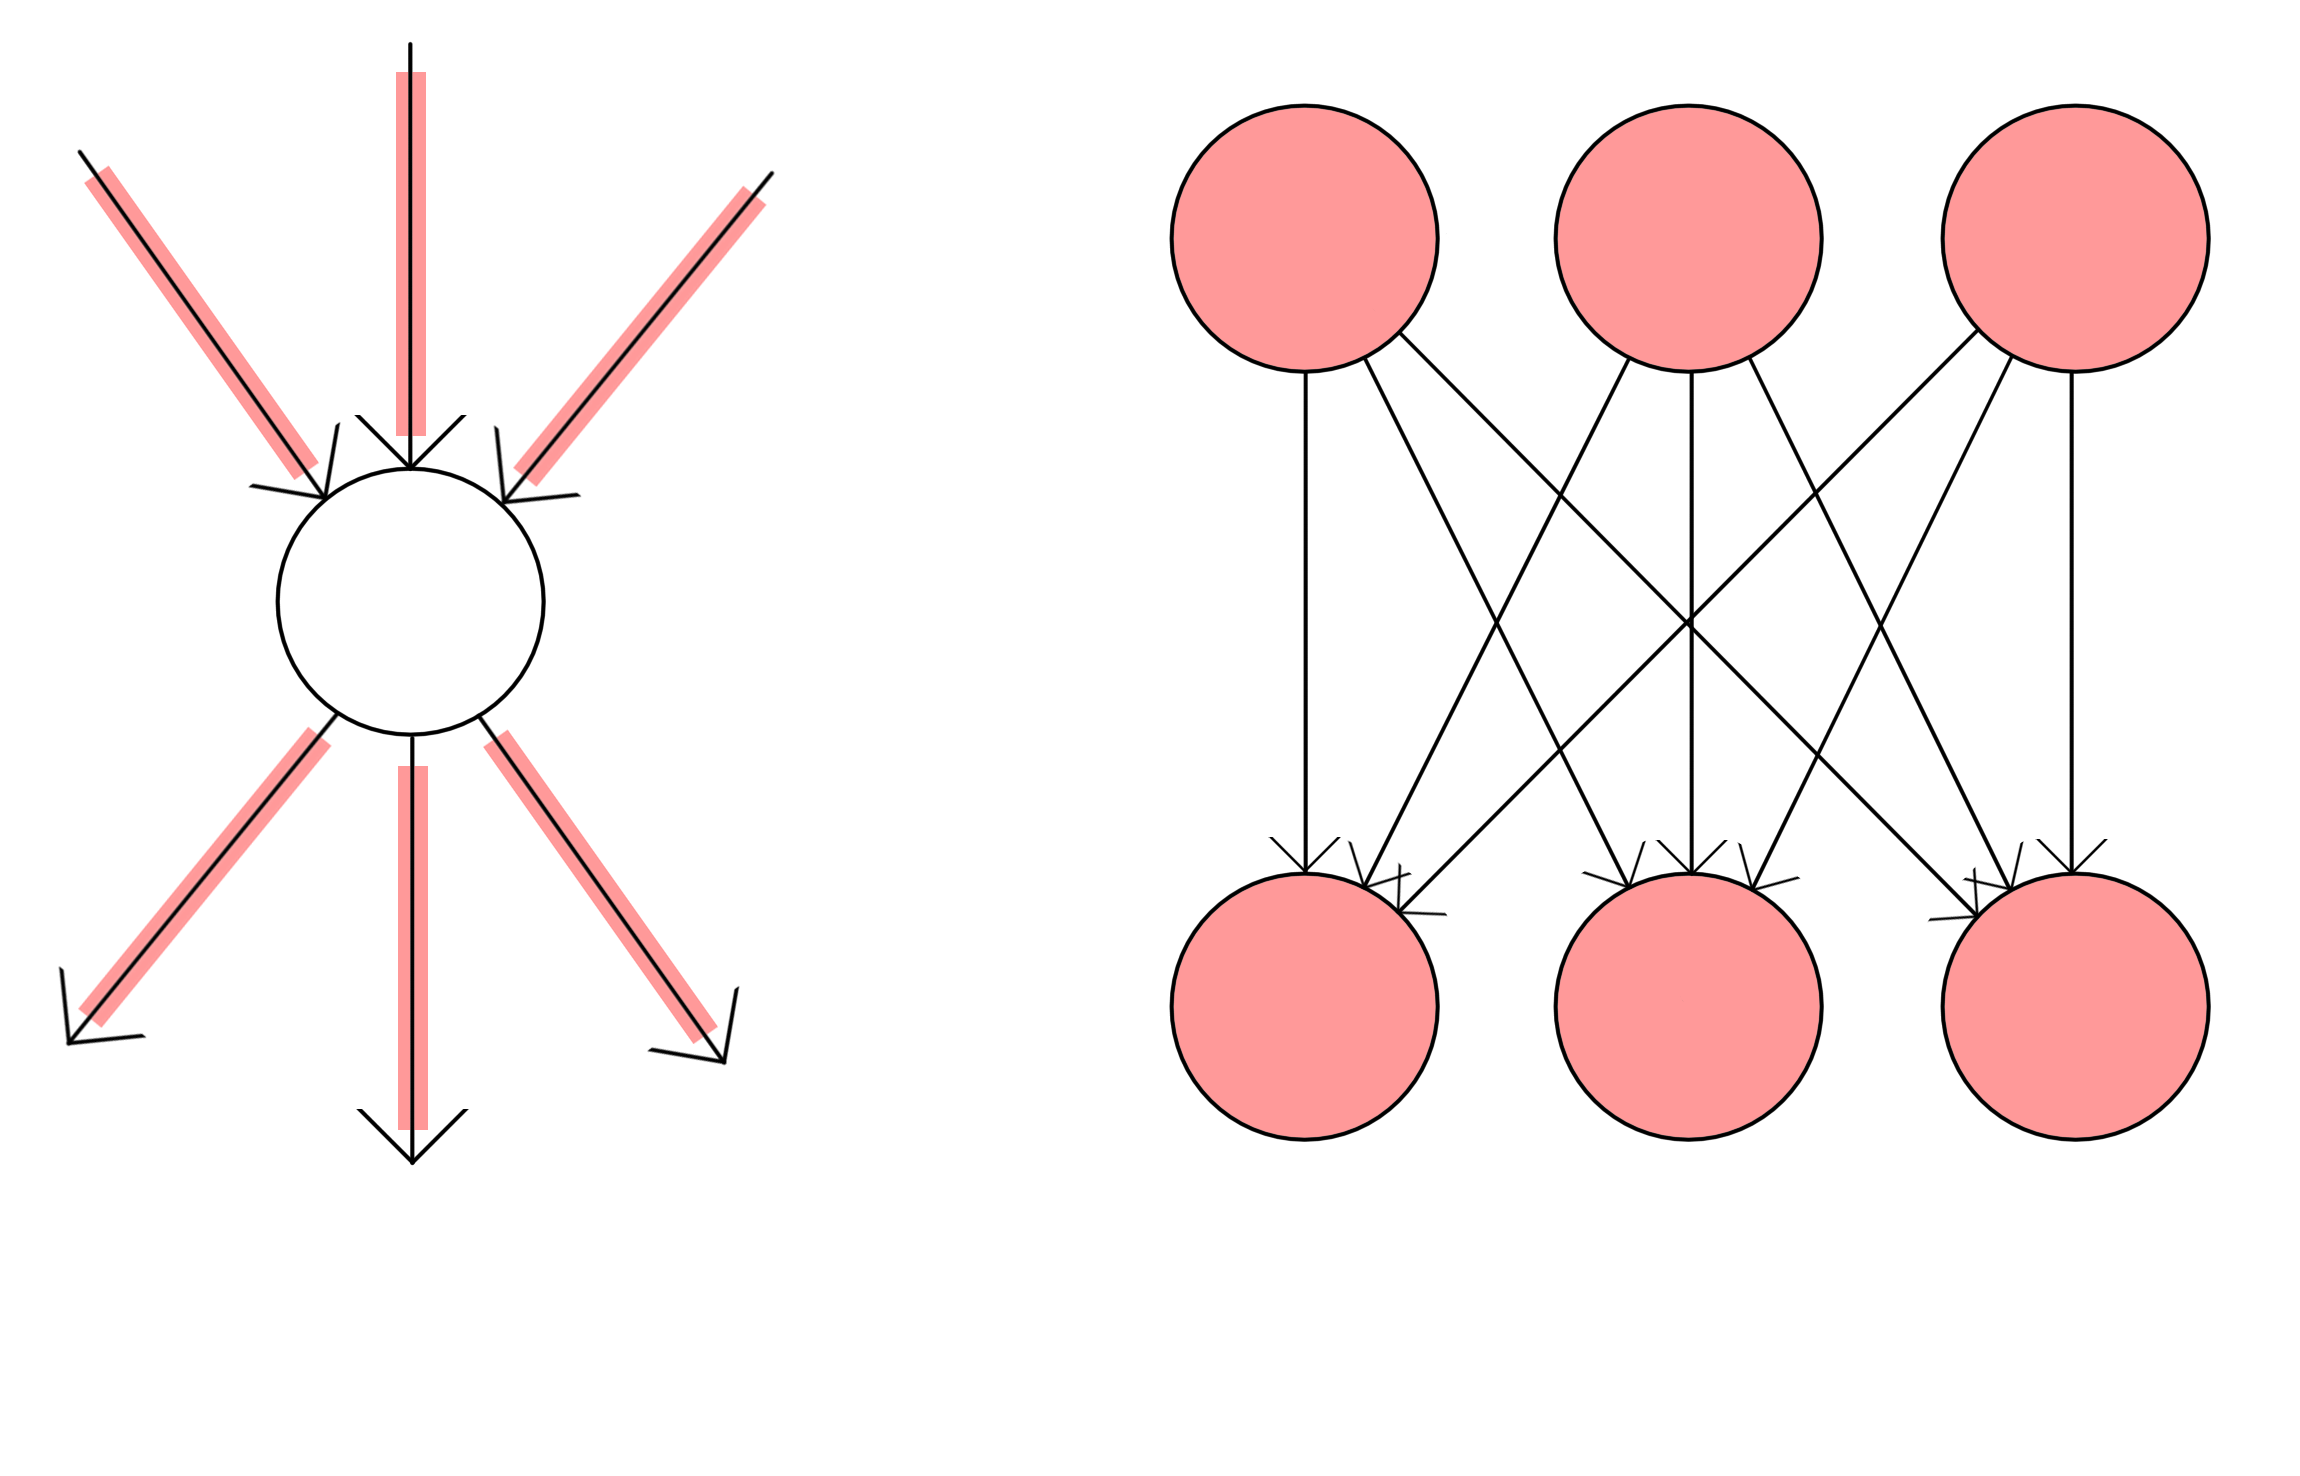
\includegraphics[width=0.75\textwidth]{figuras/ch_shift/shift-kdd.png}};
    \node at (2.2,1) {\large$D$};
    \node at (9.2,1) {\large$L(D)$};
\end{tikzpicture}
\caption{Um vértice de $D$ com $d$ arcos de mesma cor entrando e saindo corresponde a um $K_{d,d}$ monocromático em $L(D)$.}
\label{fig:shiftkdd}
\end{figure}

Note que $t=k$ (ou seja, $v$ é composto apenas de zeros) não ocorre, pois em cada vértice de $B$ entram $td$ arcos de $t$ possíveis cores, logo alguma cor ocorre pelo menos $d$ vezes, contradizendo o fato de que $v$ é composto apenas de zeros.
\end{proof}

\begin{lema}\label{shiftlema2}
Existe um subgrafo $H$ de $S_n^r$ com cintura pelo menos $g$ e contendo pelo menos uma aresta de cada $K_{d,d}$ de $S_n^r$.
\end{lema}

\begin{proof}(Lema \ref{shiftlema2})
Seja $\lambda = 1/4g$, $\theta = (g-2)/(g-1.75)$, $d = n^\theta$ e $p = d^{\lambda-1}$. Seja $H$ um subgrafo aleatório de $S_n^r$ em que cada aresta é escolhida com probabilidade $p$, e seja~$\Delta = \Delta(S_n^r) = n-r-1$.
Demonstraremos usando o Lema Local de Lovász que com probabilidade positiva $H$ tem cintura pelo menos $g$ e contém uma aresta de cada $K_{d,d}$.

Para cada circuito $C$ de $S_n^r$ com $|C| \leq g$, seja $A_C$ o evento de todas as arestas de $C$ estarem em~$H$. Então temos que \[\bbp(A_C) = p^{|C|}.\]

Para cada subgrafo $B$ isomorfo a $K_{d,d}$ de $S_n^r$, seja $A_B$ o evento de nenhuma aresta de $B$ estar em $H$. Então \[\bbp(A_B) = (1-p)^{d^2} \leq e^{pd^2} = e^{-d^{1+\lambda}}.\]

Cada circuito $C$ compartilha aresta com no máximo $|C|\Delta^{j-2}$ circuitos de comprimento $j$, e compartilha aresta com no máximo $|C|\binom{\Delta}{d}^2$ subgrafos $B$ isomorfos a $K_{d,d}$.

Cada subgrafo $B$ compartilha aresta com no máximo $d^2\Delta^{j-2}$ circuitos de comprimento $j$, e compartilha aresta com no máximo $\binom{\Delta}{d}^2$ subgrafos isomorfos a $K_{d,d}$.

Sejam $y_{|C|} = \bbp(A_C)^{1-\lambda}$ e $y_0 = y(B) = e^{-0.5d^{1+\lambda}}$. Queremos mostrar que

\begin{equation*}
\bbp(A_C) \leq y_{|C|}\left(\prod_{3\leq j\leq g}(1-y_j)^{|C|\Delta^{j-2}}\right)(1-y_0)^{|C|\binom{\Delta}{d}^2},
\end{equation*}
\begin{equation*}
\bbp(A_B)\leq y_0 \left(\prod_{3\leq j\leq g}(1-y_j)^{d^2\Delta^{j-2}}\right)(1-y_0)^{\binom{\Delta}{d}^2}.
\end{equation*}

%%%%%%%%%%%%%%%%%%%%%%%%%%%%%%%%%%%%%%%%%%%%%%%%%%%%%%%%%%%%%%%%%%%
Temos que $\Delta < n$, portanto basta mostrar que

\begin{equation}\label{shiftllleq1}
\bbp(A_C) \leq y_{|C|}\left(\prod_{3\leq j\leq g}(1-y_j)^{|C|n^{j-2}}\right)(1-y_0)^{|C|\binom{n}{d}^2},
\end{equation}
\begin{equation}\label{shiftllleq2}
\bbp(A_B)\leq y_0 \left(\prod_{3\leq j\leq g}(1-y_j)^{d^2n^{j-2}}\right)(1-y_0)^{\binom{n}{d}^2}.
\end{equation}

Para mostrar a inequação (\ref{shiftllleq1}), tomamos seu logaritmo

\[\log(\bbp(A_C)) \leq \log(\bbp(A_C)^{1-\lambda}) + \sum\limits_{3\leq j\leq g}|C|n^{j-2}\log(1-y_j)+|C|\binom{n}{d}^2\log(1-y_0).\]

Então basta mostrar que

\[|C|(\lambda-1)\log(d) \leq -(1-\lambda)^2|C|\log(d) + \sum\limits_{3\leq j\leq g}|C|n^{j-2}\log(1-y_j)+|C|\binom{n}{d}^2\log(1-y_0).\]

Podemos dividir todos os termos por $|C|$ para obter

\[(\lambda-1)\log(d) \leq -(1-\lambda)^2\log(d) + \sum\limits_{3\leq j\leq g}n^{j-2}\log(1-y_j)+\binom{n}{d}^2\log(1-y_0).\]

E reorganizando os termos, obtemos

\[(\lambda-\lambda^2)\log(d) \geq -\sum\limits_{3\leq j\leq g}n^{j-2}\log(1-y_j)-\binom{n}{d}^2\log(1-y_0).\]

Como $0.9\log(1-z) > -z$ para $z$ pequeno, então $-\log(1-z)<z/0.9$ para $z$ pequeno, então basta mostrar que

\[\lambda(1-\lambda)\log(d) \geq \sum\limits_{3\leq j \leq g}n^{j-2}\frac{y_j}{0.9} + \binom{n}{d}^2\frac{y_0}{0.9},\]

ou seja,

\[0.9\lambda(1-\lambda)\log(d) \geq \sum\limits_{3\leq j \leq g}n^{j-2}d^{-(1-\lambda)^2j} +\binom{n}{d}^2e^{-0.5d^{1+\lambda}}.\]

Como $d^{-(1-\lambda)^2j} < d^{(2\lambda-1)j}$, temos

\begin{equation}\label{shiftllleq3}
0.9\lambda(1-\lambda)\log(d) \geq \sum\limits_{3\leq j \leq g}n^{j-2}d^{(2\lambda-1)j}+\binom{n}{d}^2e^{-0.5d^{1+\lambda}}.
\end{equation}

Portanto, para mostrar a inequação (\ref{shiftllleq1}), basta mostrar a inequação (\ref{shiftllleq3}). Consideraremos separadamente os dois termos do lado direito da inequação (\ref{shiftllleq3}).

Como temos que $\binom{n}{d}^2 < (\frac{en}{d})^{2d}$, então

% $g-2+\theta/2-g\theta \leq -1$

% $2g - 4 + \theta(1-2g) \leq -2$

% $\theta(1-2g) \leq -2g+2$

% $\theta(2g-1) \geq 2g-2$

% %% or
% $(g-2)/\theta + 1/4 - g \leq -1.5$ 

% $(g-2)/\theta \leq g-1.5-1/4$

% $(g-2)/(g-1.75) \leq \theta$

\begin{equation*}
\setlength{\jot}{6pt}
\begin{aligned}
\binom{n}{d}^2e^{-0.5d^{1+\lambda}} &< \left(\frac{en}{d}\right)^{2d}e^{-0.5d^{1+\lambda}}\\ 
&= \left(\frac{e^2n^2}{d^2}e^{-0.5d^\lambda}\right)^d.
\end{aligned}
\end{equation*}

Como $d = n^\theta$, temos que

\begin{equation*}
\setlength{\jot}{6pt}
\begin{aligned}
\left(\frac{e^2n^2}{d^2}e^{-0.5d^\lambda}\right)^d 
&= \left(\frac{e^2n^2}{n^{2\theta}}e^{-0.5d^\lambda}\right)^d \\
&= \left(e^2(n^{1-\theta})^2e^{-0.5d^\lambda}\right)^d\\ 
&= \left(\frac{n^{2-2\theta}}{e^{0.5d^\lambda-2}}\right)^d. 
%&< \left(\frac{36}{e^{0.5d^\lambda}}\right)^d.
\end{aligned}
\end{equation*}

Como $g\geq 3$, temos que $\theta \geq 0.8$, logo

\begin{equation*}
\setlength{\jot}{6pt}
\begin{aligned}
\left(\frac{n^{2-2\theta}}{e^{0.5d^\lambda-2}}\right)^d 
&\leq \left(\frac{n^{0.4}}{e^{0.5d^\lambda-2}}\right)^d\\
&= \left(\frac{n^{0.4}}{e^{0.5n^{\theta\lambda}-2}}\right)^d
\end{aligned}
\end{equation*}

Se $n$ é tal que

\[\theta\lambda = \frac{g-2}{4g(g-1.75)} \geq \frac{\log(\log(n))}{\log(n)},\]

então 

\[e^{0.5n^{\theta\lambda}-2} \geq n^{0.4}.\]

Pois temos que

\begin{equation*}
\setlength{\jot}{6pt}
\begin{aligned}
n^{\theta\lambda} &\geq \log(n)\\
&= 0.8\log(n) + 0.2\log(n).
\end{aligned}
\end{equation*}

E note que para tal $n$, temos que $0.2\log(n) \geq 4$, logo

\[n^{\theta\lambda} \geq 0.8\log(n) + 4.\]

Ou seja, temos que

\[0.5n^{\theta\lambda} - 2 \geq 0.4\log(n),\]

e logo temos que

\[e^{0.5n^{\theta\lambda}-2} \geq n^{0.4}.\]

Então

\begin{equation*}
\setlength{\jot}{6pt}
\begin{aligned}
\left(\frac{n^{0.4}}{e^{0.5n^{\theta\lambda}-2}}\right)^d
&\leq 1^d\\
&= 1.
\end{aligned}
\end{equation*}

% Logo, para $n$ suficientemente grande, temos que

% \begin{equation*}
% \setlength{\jot}{6pt}
% \begin{aligned}
% \left(\frac{n^{0.4}}{e^{0.5n^{\theta\lambda}-2}}\right)^d &
% \leq 1^d\\
% &= 1.
% \end{aligned}
% \end{equation*}

Portanto, concluímos que

\begin{equation}\label{shiftlllaux1}
\binom{n}{d}^2e^{-0.5d^{1+\lambda}} < 1.
\end{equation}

% Em particular, basta que

% \[0.5n^{\theta\lambda}-2 \geq 0.4\log(n).\]

% Equivalentemente, basta que

% \[n^{\theta\lambda} \geq 0.8\log(n) + 4.\]

% Se $0.2\log(n) \geq 4$, ou seja, se $n \geq e^{20}$, basta que $n$ seja tal que

% \[n^{\theta\lambda} \geq \log(n).\]

% Logo, basta que

% \[\theta\lambda\log(n) \geq \log(\log(n)).\]

% Então, se 

%Em particular, como $n^c \leq e^n$ para todo $n>0$ e $c\in (0,1)$, para que a desigualdade (\ref{shiftlllaux1}) seja verdadeira basta que

%%%%%%%%%%%%%%%%%%%%%%%%%%%%%%%%%%%%%%%%%%%%%%%%%%%%%%%%%%%%%%%%%%%
%%
%% Se n^c <= e^n, pra n >= 0 e c in (0,1), basta que 0.5d^\lambda - 2 > 0.
%% Não parece estar certo.....
%%
%%%%%%%%%%%%%%%%%%%%%%%%%%%%%%%%%%%%%%%%%%%%%%%%%%%%%%%%%%%%%%%%%%%

Como $\lambda g = 1/4$ e $n = d^{1/\theta}$, temos também que

\begin{equation*}
\setlength{\jot}{6pt}
\begin{aligned}
\sum\limits_{3\leq j \leq g}n^{j-2}d^{(2\lambda-1)j} 
&< gn^{g-2}d^{(2\lambda-1)g} \\
&\leq gd^{(g-2)/\theta}d^{(2\lambda-1)g} \\
&= gd^{g-1.75}d^{2\lambda g-g} \\
&= gd^{-1.75}d^{2\lambda g} \\
&= gd^{-1.75}d^{0.5} \\
&= gd^{-1.25}.
\end{aligned}
\end{equation*}

% \begin{equation*}
% \setlength{\jot}{6pt}
% \begin{aligned}
% \sum\limits_{3\leq j \leq g}\Delta^{j-2}d^{(2\lambda-1)j} 
% &\leq \Delta^{g-2}d^{(2\lambda-1)g} \\
% &\leq (2d)^{g-2}d^{(2\lambda-1)g} \\
% &< 2^gd^{g-2}d^{(2\lambda-1)g} \\
% &= 2^gd^{-2}d^{2\lambda g} \\
% &= 2^gd^{-2}d^{0.5} \\
% &= 2^gd^{-1.5}.
% \end{aligned}
% \end{equation*}

Então concluímos que

\begin{equation}\label{shiftlllaux2}
\sum\limits_{3\leq j \leq g}n^{j-2}d^{(2\lambda-1)j} < gd^{-1.25}.
\end{equation}

Aplicando (\ref{shiftlllaux1}) e (\ref{shiftlllaux2}) na inequação  (\ref{shiftllleq3}), basta que

\[0.9\lambda(1-\lambda)\log(d) \geq gd^{-1.25} + 1.\]

Como $d^{-1.25} \leq 1$ para todo $d\geq 1$, basta que

\[0.9\lambda(1-\lambda)\log(d) \geq g + 1.\]

Logo, se também temos que

\begin{equation*}
\setlength{\jot}{6pt}
\begin{aligned}
n &\geq \exp\left(\frac{g-1}{0.9\lambda(1-\lambda)\theta}\right)\\
&= \exp\left(\frac{(g-1)(g-1.75)16g^2}{0.9(g-2)(4g-1)}\right),
\end{aligned}
\end{equation*}
então a desigualdade (\ref{shiftllleq1}) é verdadeira.

De forma semelhante, para mostrar (\ref{shiftllleq2}), tomamos o logaritmo

\[\log(\bbp(A_B))\leq \log(y_0) + \sum\limits_{3\leq j \leq g}d^2n^{j-2}\log(1-y_j)+ \binom{n}{d}^2\log(1-y_0).\]

Então basta mostrar que

\[-d^{1+\lambda} \leq -0.5d^{1+\lambda} + \sum\limits_{3\leq j \leq g}d^2n^{j-2}\log(1-y_j)+ \binom{n}{d}^2\log(1-y_0).\]

Reordenando os termos, obtemos

\[0.5d^{1+\lambda} \geq - \sum\limits_{3\leq j \leq g}d^2n^{j-2}\log(1-y_j)- \binom{n}{d}^2\log(1-y_0).\]

Como $-\log(1-z) < z/0.9$ para $z$ pequeno, temos

\[0.5d^{1+\lambda} \geq \sum\limits_{3\leq j \leq g}d^2n^{j-2}\frac{y_j}{0.9} + \binom{n}{d}^2\frac{y_0}{0.9},\]

ou seja,

%\[0.45d^{1+\lambda} \geq \sum\limits_{3\leq j \leq g}d^2\Delta^{j-2}y_j + \binom{\Delta}{d}^2y_0.\]

\[0.45d^{1+\lambda} \geq \sum\limits_{3\leq j \leq g}d^2n^{j-2}d^{-(1-\lambda)^2j} + \binom{n}{d}^2e^{-0.5d^{1+\lambda}}.\]

Como $d^{-(1-\lambda)^2j} < d^{(2\lambda-1)j}$, temos

\begin{equation}\label{shiftllleq4}
0.45d^{1+\lambda} \geq \sum\limits_{3\leq j \leq g}d^2n^{j-2}d^{(2\lambda-1)j} + \binom{n}{d}^2e^{-0.5d^{1+\lambda}}.
\end{equation}

Logo para mostrar (\ref{shiftllleq2}), basta mostrar que (\ref{shiftllleq4}) vale.

Por (\ref{shiftlllaux2}), temos que

\begin{equation*}
\setlength{\jot}{6pt}
\begin{aligned}
\sum\limits_{3\leq j \leq g}d^2n^{j-2}d^{(2\lambda-1)j} &= d^2\sum\limits_{3\leq j \leq g}n^{j-2}d^{(2\lambda-1)j} \\
&\leq d^2gd^{-1.25} \\
&= gd^{0.75}.
\end{aligned}
\end{equation*}

E por (\ref{shiftlllaux1}), temos que

\[\binom{n}{d}^2e^{-0.5d^{1+\lambda}} < 1.\]

Então para mostrar (\ref{shiftllleq4}), basta que 

\[0.45d^{1+\lambda} \geq gd^{0.75} + 1.\]

Como $d^{0.75} \geq 1$ para todo $d \geq 1$, então basta que

\begin{equation*}
\setlength{\jot}{6pt}
\begin{aligned}
0.45d^{1+\lambda} &\geq gd^{0.75} + d^{0.75}\\
&= (g+1)d^{0.75}.
\end{aligned}
\end{equation*}

Logo, se

\[d^{0.25+\lambda} = n^{\theta(0.25+\lambda)} \geq \frac{g+1}{0.45},\]

então a inequação (\ref{shiftllleq2}) é verdadeira.

%Como $2^g$ é constante, note que o lado esquerdo da inequação tem crescimento maior do que o lado direito, e logo para $d$ suficientemente grande a inequação vale. 

%E como o lado esquerdo da inequação é crescente com limite tendendo para infinito, e o lado direito é decrescente, para $d$ suficientemente grande, a inequação vale.

Logo temos que (\ref{shiftllleq1}) e (\ref{shiftllleq2}) são verdadeiras para $n$ suficientemente grande.

Portanto, pelo Lema Local de Lovász, a probabilidade de nenhum dos eventos $A_C$ e $A_B$ ocorrerem é positiva, ou seja, existe um subgrafo de $S_n^r$ com cintura maior que $g$ e com pelo menos uma aresta de cada $K_{d,d}$.

\end{proof}

Mostraremos agora que os \textit{shift graphs} respeitam a conjectura de Erd\H{o}s e Hajnal.

\begin{proof}(Teorema \ref{shiftteo})
Seja $D$ uma orientação transitiva de $K_n$, e sejam $k,g$ os parâmetros da conjectura de Erd\H{o}s e Hajnal.

Note que $S_{n-1}^r$ é subgrafo de $S_n^r$, logo $\chi(S_{n-1}^r) \leq \chi(S_n^r)$, então basta mostrar que existe algum~$n_0 := n_0(k,g)$ tal que $S_{n_0}^r$ contém um subgrafo com número cromático pelo menos $k$ e cintura pelo menos $g$.

Pelo Lema \ref{shiftlema2}, existe um subgrafo de $S_n^r$ com cintura pelo menos $g$ e que contenha pelo menos uma aresta de cada $K_{d,d}$. Seja $H$ um tal subgrafo.

Suponha por contradição que o número cromático de $H$ é limitado por uma constante $t$, logo uma coloração própria de $H$ corresponde a uma $t$-coloração de $S_n^r$ sem $K_{d,d}$ monocromático, e portanto, pela Afirmação \ref{shiftafirm1}, corresponde a uma $t$-coloração de $L^r(D)$ sem $K_{d,d}$ monocromático.

Pelo Lema \ref{shiftlema1}, existe uma $2^t$-coloração de $L^{r-1}(D)$ sem $K_{td,td}$ monocromático. Aplicando o lema novamente, temos que existe uma $2^{2^t}$-coloração de $L^{r-2}(D)$ sem $K_{2^ttd,2^ttd}$ monocromático.

\begin{figure}[H]
\centering
\begin{tikzpicture}

    \node (D0) at (0,0) {$L^r(D)$};
    \draw[dotted] (D0) circle (1);
    \node (D1) at (5,0) {$L^{r-1}(D)$};
    \draw[dotted] (D1) circle (1);
    \node (D2) at (10,0) {$L^{r-2}(D)$};
    \draw[dotted] (D2) circle (1);
    \node[below=of D0] {
        \begin{tabular}{c}
        $t$-coloração sem \\ $K_{d,d}$ monocromático 
        \end{tabular}
    };
    \node[below=of D1] {
        \begin{tabular}{c}
        $2^t$-coloração sem \\ $K_{td,td}$ monocromático 
        \end{tabular}
    };
    \node[below=of D2] {
        \begin{tabular}{c}
        $2^{2^t}$-coloração sem \\ $K_{2^ttd,2^ttd}$ monocromático 
        \end{tabular}
    };
    \draw[->] (1.25,0) to (3.75,0);
    \draw[->] (6.25,0) to (8.75,0);
    \node at (2.5,0.3) {Lema};
    \node at (7.5,0.3) {Lema};
\end{tikzpicture}
\caption{Aplicações sucessivas do Lema.}
\label{fig:shiftlemmaap}
\end{figure}

Então, aplicando o lema $r$ vezes temos que existe uma $t'$-coloração de $L^0(D)$ sem $K_{d',d'}$ monocromático, para algum $t'$ e algum $d'$. 

\begin{figure}[H]
\centering
\begin{tikzpicture}

    \node (D0) at (0,0) {};
    \draw[dotted] (D0) circle (1);
    \node (D1) at (5,0) {};
    \draw[dotted] (D1) circle (1);
    \node (D2) at (8.5,0) {$\cdots$};
    \node (D3) at (12,0) {};
    \draw[dotted] (D3) circle (1);
    \node[xshift=-0.2cm, yshift=0.1cm] (DH) at (D0) {$H$};
    \draw[dotted] (DH) circle (0.7);
    \node[above=of D0] {$L^r(D)$};
    \node[above=of D1] {$L^{r-1}(D)$};
    \node[above=of D3] {$L^0(D)$};
    \node[below=of D0] {
        \begin{tabular}{c}
        $t$-coloração sem \\ $K_{d,d}$ monocromático 
        \end{tabular}
    };
    \node[below=of D1] {
        \begin{tabular}{c}
        $2^t$-coloração sem \\ $K_{td,td}$ monocromático 
        \end{tabular}
    };
    \node[below=of D3] {
        \begin{tabular}{c}
        $t'$-coloração sem \\ $K_{d',d'}$ monocromático 
        \end{tabular}
    };
    \draw[->] (1.25,0) to (3.75,0);
    \draw[->] (6.25,0) to (7.5,0);
    \draw[->] (9.5,0) to (10.75,0);
    \node at (2.5,0.3) {Lema};
    \node at (6.825,0.3) {Lema};
    \node at (10.025,0.3) {Lema};
\end{tikzpicture}
\caption{A coloração de $H$ corresponde a uma $t$-coloração de $L^r(D)$ sem $K_{d,d}$ monocromático, e por meio de aplicações sucessivas do Lema, obtemos uma $t'$-coloração de $L^0(D)$ sem $K_{d',d'}$ monocromático.}
\label{fig:shiftlemmasequence}
\end{figure}

% \begin{figure}[H]
% \centering
% \begin{tikzpicture}
%     \node[anchor=south west,inner sep=0] at (0,0) {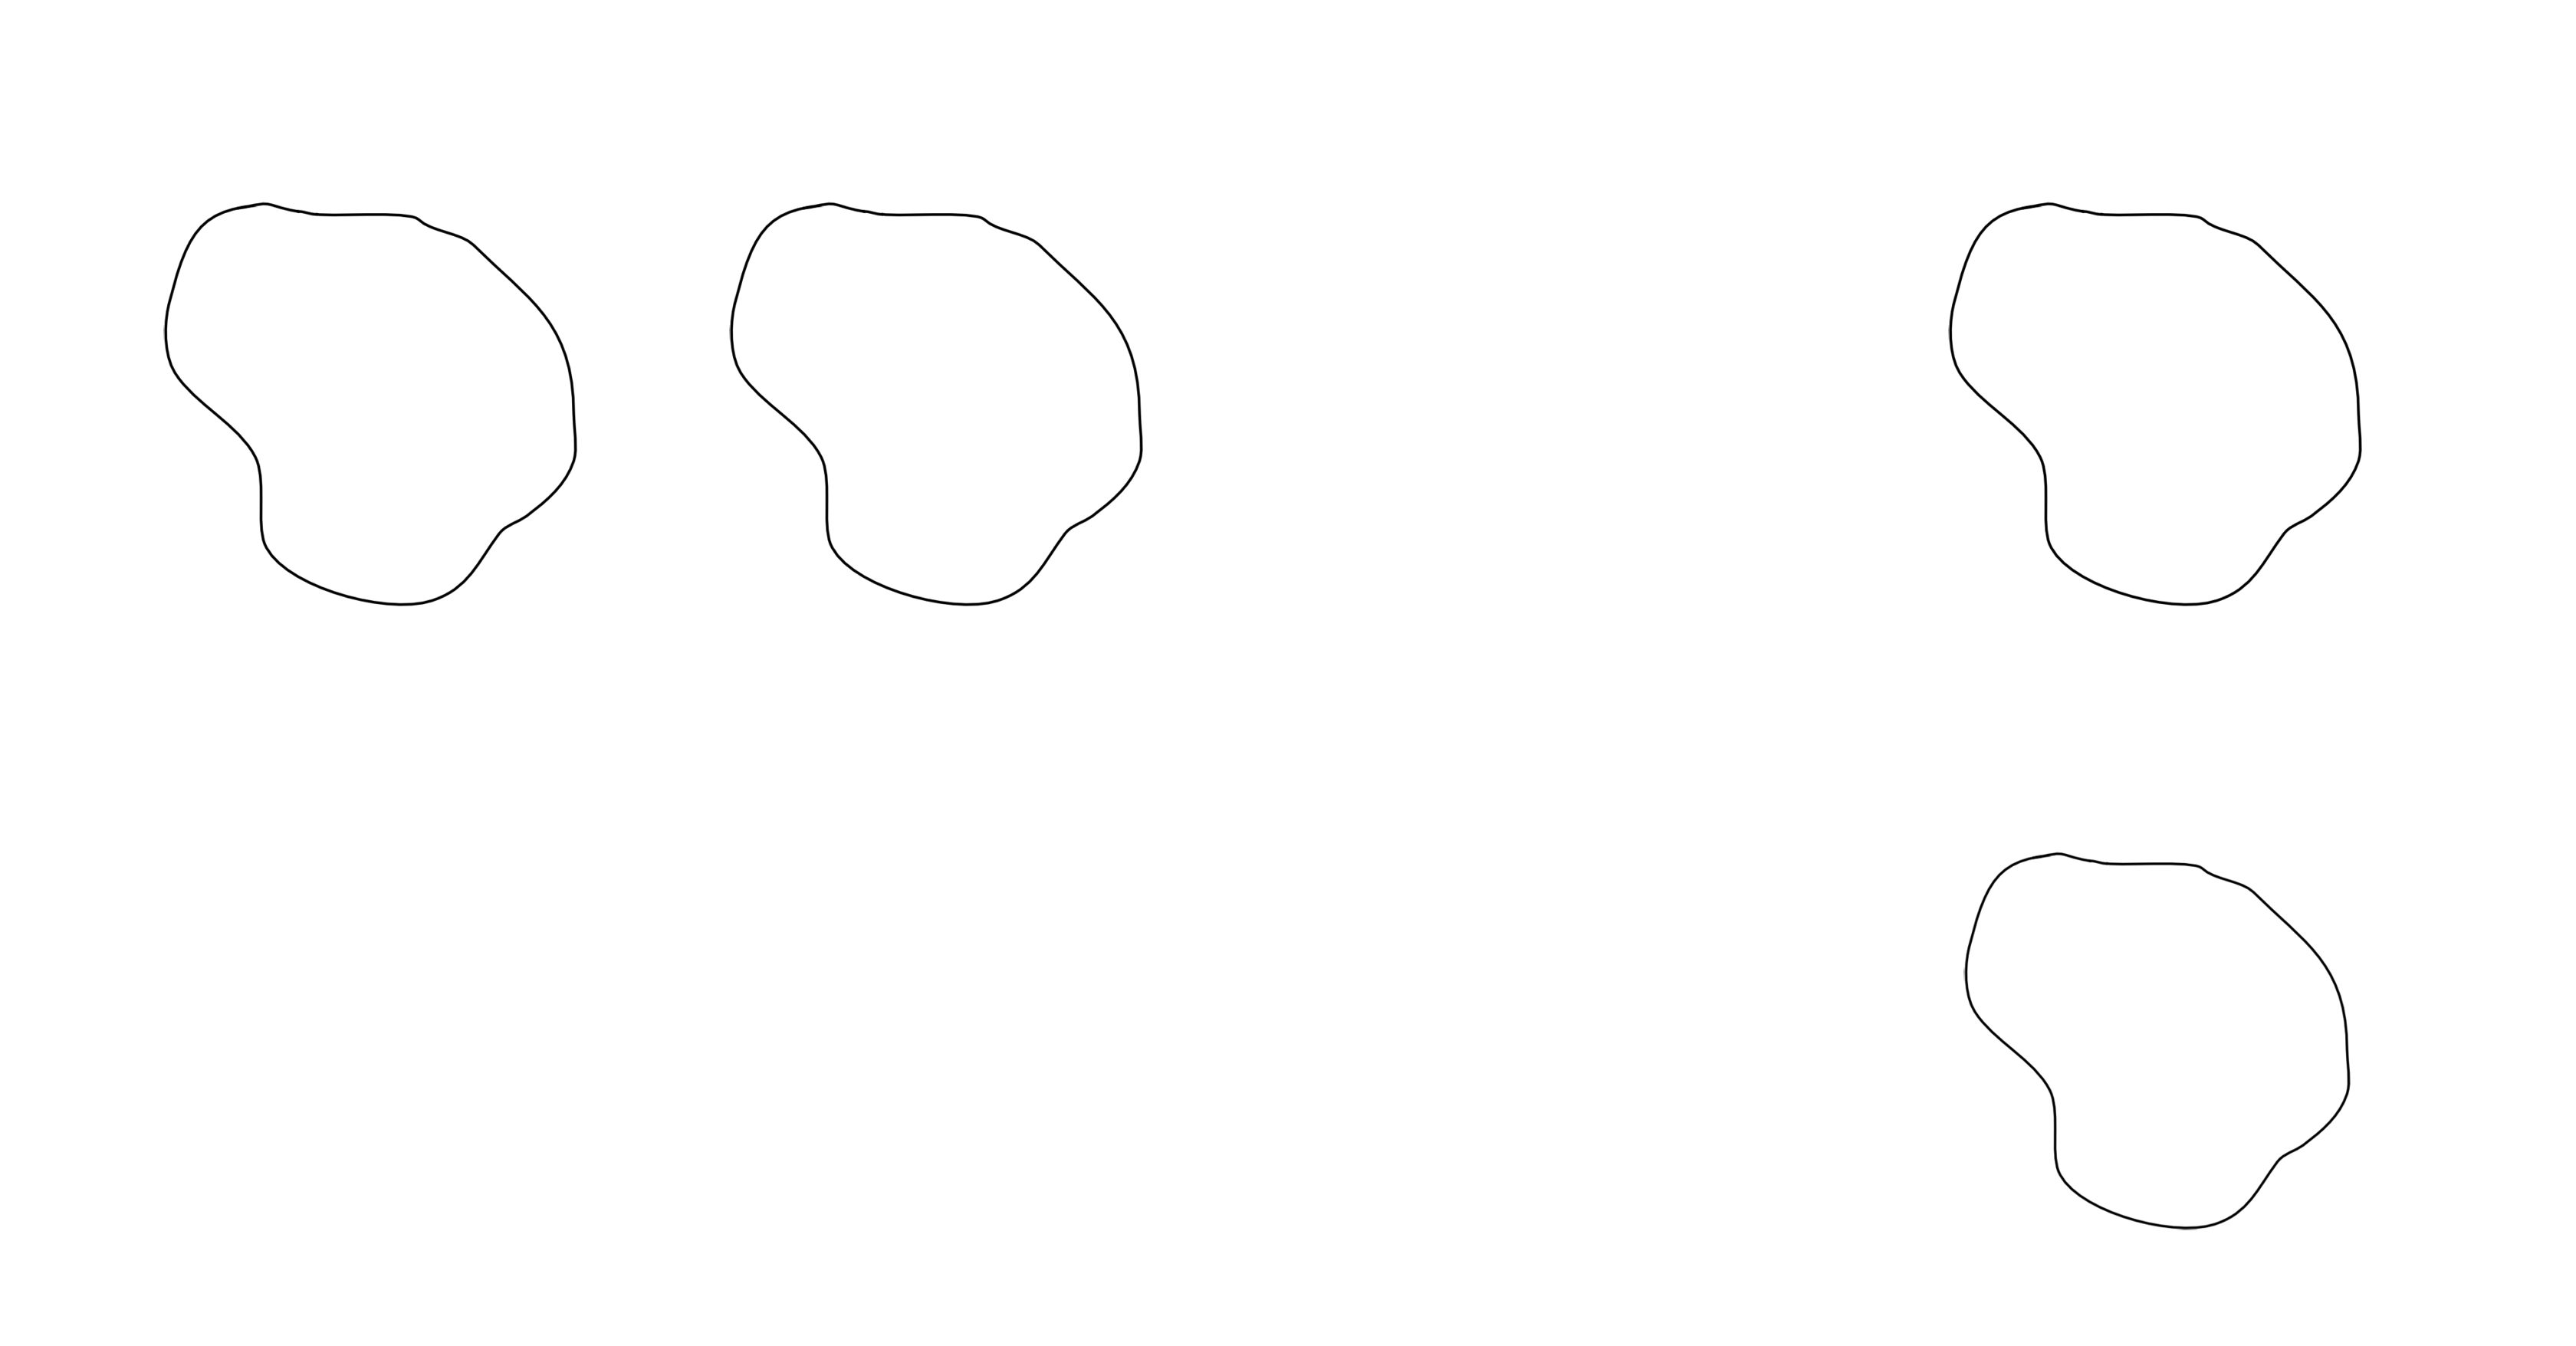
\includegraphics[width=0.95\textwidth]{figuras/ch_shift/shift-sequence.png}};
%     \node at (2.3,5.8) {\large$D$};
%     \node at (5.8,5.8) {\large$L^1(D)$};
%     \node at (13.25,5.8) {\large$L^r(D)$};
%     \node at (13.1,1.9) {\large$H$};
%     \node at (9.52,5.8) {\Large$\cdots$};
%     \draw[->](11.9,2.1) to [bend left,looseness=1.2] node [left]{Coloração} (11.9,5.6);
%     \draw[->](5.3,7) to [bend right,looseness=1] node [above]{Lema} (2.8,7);
%     \draw[->](8.8,7) to [bend right,looseness=1] node [above]{Lema} (6.3,7);
%     \draw[->](12.75,7) to [bend right,looseness=1] node [above]{Lema} (10.25,7);
% \end{tikzpicture}
% \caption{A coloração de $H$ corresponde a uma $t$-coloração de $L^r(D)$ sem $K_{d,d}$ monocromático, e por meio de aplicações sucessivas do Lema, obtemos uma $t'$-coloração de $D$ sem $K_{t',t'}$ monocromático.}
% \label{fig:shiftsequence}
% \end{figure}

Mas $L^0(D) = D$, e note que todo conjunto de $2d'$ vértices de $D$ é um $K_{d',d'}$, então concluímos que existe uma $t'$ coloração de $D$ tal que nenhuma cor ocorre $2d'$ vezes, uma contradição pois se~$n \geq t'(2d'-1)+1$, pelo princípio da casa dos pombos, alguma cor ocorre pelo menos $2d'$ vezes.

Portanto o número cromático de $H$ não é limitado por constante.
\end{proof}

%%%%%%%%%%%%%%%%%%%%%%%%%%%
%% Talvez escrever type graphs em um capítulo separado?
%%%%%%%%%%%%%%%%%%%%%%%%%%%

\section{\textit{Type Graphs}}

Os \textit{shift graphs} tem como vértices subconjuntos de $[n]$, e dois vértices são adjacentes se suas ``extremidades'' coincidem. Os \textit{type graphs} generalizam a regra de adjacência, de forma que dois vértices são adjacentes se os elementos de seus conjuntos respeitam algum padrão de pertinência, dizemos que tal padrão é um \textit{type}.

\begin{definicao}
Sejam $A_1, A_2$ $m$-subconjuntos de $[n]$. O \textit{type} do par $(A_1,A_2)$, denotado $\tau(A_1,A_2)$, é a sequência $(z_1, z_2,\cdots,z_l)$, onde $l := |A_1\cup A_2|$ e

\[ z_i = \begin{cases} 
      1 & \text{se } (A_1\cup A_2)_i \in A_1\setminus A_2\\
      2 & \text{se } (A_1\cup A_2)_i \in A_2\setminus A_1\\
      3 & \text{se } (A_1\cup A_2)_i \in A_1\cap A_2.
   \end{cases}
\]

Dizemos que $l$ é o comprimento e $m$ é a largura do \textit{type}.
\end{definicao}

\begin{figure}[H]
\centering
\begin{tikzpicture}[-latex ,auto ,node distance =0.7cm and 5cm, on grid,semithick ,state/.style ={circle, draw, text=white , minimum width =0.2 cm}]
    \node[circle, draw=black] at (0,3) {$d$};
    \node[circle, draw=black] at (0,4) {$b$};
    \node[circle, draw=black] at (0,5) {$a$};
    \draw (0,4) ellipse (0.75 and 1.6);
    \node at (0,6) {$A_1$};
    
    \node[circle, draw=black] at (8,3) {$e$};
    \node[circle, draw=black] at (8,4) {$c$};
    \node[circle, draw=black] at (8,5) {$b$};
    \draw (8,4) ellipse (0.75 and 1.6);
    \node at (8,6) {$A_2$};
    
    \node[circle, draw=black] at (2,1.5) {$a$};
    \node[circle, draw=black] at (3,1.5) {$b$};
    \node[circle, draw=black] at (4,1.5) {$c$};
    \node[circle, draw=black] at (5,1.5) {$d$};
    \node[circle, draw=black] at (6,1.5) {$e$};
    \draw (4,1.5) ellipse (2.6 and 0.6);
    \node at (0,1.5) {$A_1\cup A_2$};
    
    \node at (0,0) {$\tau(A_1, A_2) =$};
    \node at (1.5,0) {$($};
    \node at (2.1,0) {$1,$};
    \node at (3.1,0) {$3,$};
    \node at (4.1,0) {$2,$};
    \node at (5.1,0) {$1,$};
    \node at (6,0) {$2$};
    \node at (6.5,0) {$)$};
    
    \draw[->] (2,1.8) to (1.6,2.5);
    \draw[->] (3,1.85) to (2.6,2.5);
    \draw[->] (3,1.85) to (3.4,2.5);
    \draw[->] (4,1.8) to (4.4,2.5);
    \draw[->] (5,1.85) to (4.6,2.5);
    \draw[->] (6,1.8) to (6.4,2.5);
\end{tikzpicture}
\caption{O \textit{type} dos conjuntos $A_1$ e $A_2$, assumindo que $a<b<c<d<e$.}
\label{fig:typeexample}
\end{figure}

Note que $m = |\{i : z_i \in \{1,3\}\}| = |\{i : z_i \in \{2,3\}\}|$.

\begin{definicao}
Um \textit{type graph} $G(n,\tau)$, onde $\tau$ é um \textit{type} de comprimento $l$ e largura $m$, é um grafo cujos vértices são os $m$-subconjuntos de $[n]$, e dois vértices $v$ e $w$ são adjacentes se e somente se $\tau(v,w) = \tau$.
\end{definicao}

\begin{figure}[H]
\centering
\begin{tikzpicture}[-latex ,auto ,node distance =0.7cm and 5cm, on grid,semithick ,state/.style ={circle, draw, text=white , minimum width =0.2 cm}]
    \node[circle, draw=black] (A) at (0,1) {$1,4,5$};
    \node[circle, draw=black] (B) at (0,4) {$2,4,7$};
    \node[circle, draw=black] (C) at (0,7) {$1,4,6$};
    \node[circle, draw=black] (D) at (3,4) {$3,4,7$};
    
    \draw[-] (A) to (B);
    \draw[-] (B) to (C);
    \draw[-] (A) to (D);
    \draw[-] (C) to (D);
\end{tikzpicture}
\caption{Alguns vértices de um \textit{type graph} com \textit{type} $(1,2,3,1,2).$}
\label{fig:typegraphexample}
\end{figure}

O \textit{type graph} $G(n,(1,3,2))$ é isomorfo ao \textit{shift graph} $S_n$, e o \textit{type graph} $G(n, (1,3,\cdots,3,2))$, com $r$ números $3$, é isomorfo ao \textit{shift graph} $S_n^r$.

Uma generalização natural dos \textit{shift graphs}, proposta em \cite{avart2014generalized}, são os \textit{type graphs} cujos \textit{types} são como o definido a seguir.

\begin{definicao}
O \textit{type} $\sigma_{a,b}$ é a sequência composta por $a$ números $1$, seguidos por $b$ números $3$, seguidos por $a$ números $2$.
\end{definicao}

Note que o \textit{type} $\sigma_{a,b}$ tem comprimento $2a+b$ e largura $a+b$.

\begin{definicao}
Seja $A$ um conjunto. Denote por $min_i(A)$ o conjunto dos $i$ menores elementos de $A$.

Analogamente, denote por $max_i(A)$ o conjunto dos $i$ maiores elementos de $A$.
\end{definicao}

\begin{teorema}\label{typetheorem1}
Se $a\geq b$, o \textit{type graph} $G(a(n-1)+b, \sigma_{a,b})$ contém o \textit{shift graph} $S_n$ como subgrafo.
\end{teorema}
%%%%%%%%%%%%%%%%%
% Talvez G(an, sigma) basta
%%%%%%%%%%%%%%%%%

\begin{proof}(Teorema \ref{typetheorem1})
Sejam $a,b$ fixos, $a \geq b$, e seja $G = G(a(n-1)+b, \sigma_{a,b})$. Considere as sequências

\begin{equation*}
\setlength{\jot}{6pt}
\begin{aligned}
s_i &= (i-1)a+1,\ (i-1)a+2,\ \cdots,\ (i-1)a+b, & i\in [1,n] \\
t_i &= (i-1)a+b+1,\ (i-1)a+b+2,\ \cdots,\ ia, & i\in [1,n-1].
\end{aligned}
\end{equation*}

Ou seja, $s_i$ é a sequência composta por todos os elementos entre $(i-1)a + 1$ até $(i-1)a+b$, e~$t_i$ é a sequência composta por todos os elementos entre $(i-1)a + b+1$ até $ia$.

Denote por $(s_i,s_j)$, para $1\leq i < j \leq n$, os vértices de $G$ da forma \[s_i,t_i,s_j = ((i-1)a+1,\cdots, ia, (j-1)a+1,\cdots, (j-1)a+b).\]

% \begin{figure}[H]
% \centering
% \begin{tikzpicture}
%     \node at (-2,0) {$(s_i,s_j) =$};
%     \node at (0,0) {$s_i, t_i, s_j$};
%     \node at (0,3) {$(i-1)a+1,\cdots, (i-1)a+b,(i-1)a+b+1,\cdots, ia, (j-1)a+1, \cdots,(j-1)a+b$};
    
%     \draw [decorate,decoration={brace,amplitude=5,mirror}] (-7,2.75) to (-2,2.75);
    
%     \draw[-] (0,0.3) to (0,2.7);
% \end{tikzpicture}
% \caption{Alguns vértices de um \textit{type graph} com \textit{type} $(1,2,3,1,2).$}
% \label{fig:typesequence1}
% \end{figure}

Seja $H$ o subgrafo induzido pelos vértices $(s_i,s_j), 1\leq i<j\leq n$. Note que dois vértices $(s_i,s_j)$ e $(s_k,s_l)$ são adjacentes se $s_i = s_l$ ou $s_j = s_k$, ou seja, se $i=l$ ou $j=k$.

% \begin{figure}[H]
% \centering
% \begin{tikzpicture}[-latex ,auto ,node distance =0.7cm and 5cm, on grid,semithick ,state/.style ={circle, draw, text=white , minimum width =0.2 cm}]
%     \node[circle, draw=black] (A) at (0,0) {$(s_i,s_j)$};
%     \node at (0,2) {$\cdots,(j-1)a+1, \cdots,(j-1)a+b$};
% \end{tikzpicture}
% \caption{}
% \label{fig:typegraphH1}
% \end{figure}

Temos que $H$ é um grafo da seguinte forma

\begin{equation*}
\setlength{\jot}{6pt}
\begin{aligned}
V(H) &= \{(s_i,s_j) : 1\leq i<j\leq n\}\\
E(H) &= \{vw : v,w\in V(H),\ max(v) = min(w)\}.
\end{aligned}
\end{equation*}

E note que o \textit{shift graph} $S_n$ é da forma

\begin{equation*}
\setlength{\jot}{6pt}
\begin{aligned}
V(S_n) &= \{(i,j) : 1\leq i<j\leq n\}\\
E(S_n) &= \{vw : v,w\in V(S_n),\ max(v) = min(w)\}.
\end{aligned}
\end{equation*}

Temos então que $H$ é isomorfo a $S_n$. Logo, temos que $G$ contém o \textit{shift graph} $S_n$ como subgrafo.
\end{proof}

\begin{corolario}\label{typecor1}
Se $a\geq b$, a família dos \textit{type graphs} com \textit{type} $\sigma_{a,b}$ respeita a conjectura de Erd\H{o}s e Hajnal.
\end{corolario}

\begin{proof}(Corolário \ref{typecor1})
Sejam $k,g$ os parâmetros da conjectura de Erd\H{o}s e Hajnal. Seja~$n_0$ o menor inteiro tal que $S_{n_0}$ contém um subgrafo com número cromático pelo menos $k$ e cintura pelo menos $g$.

Tome $\sigma_{a,b}$ fixo, com $a\geq b$, e seja $n := a(n_0-1)+b$. Pelo Teorema \ref{typetheorem1}, o \textit{type graph} $G(n,\sigma_{a,b})$ contém $S_{n_0}$ como subgrafo, e logo contém um subgrafo com número cromático pelo menos $k$ e cintura pelo menos $g$.

E note que para qualquer \textit{type} $\tau$, $G(m,\tau)$ contém $G(m-1,\tau)$ como subgrafo, logo todo grafo~$G(N,\sigma_{a,b})$ com $N \geq n$ contém um subgrafo com número cromático pelo menos $k$ e cintura pelo menos $g$.
\end{proof}

\begin{teorema}\label{typetheorem2}
Se $d$ é divisor comum de $a$ e $b$, então o \textit{type graph} $G(dn,\sigma_{a,b})$ contém o \textit{type graph}~$G(n,\sigma_{a/d,b/d})$ como subgrafo.
\end{teorema}

\begin{proof}(Teorema \ref{typetheorem2})
Sejam $a,b$ e $d$ inteiros fixos, onde $d$ é divisor comum de $a$ e $b$, e seja~$G = G(dn,\sigma_{a,b})$.

Considere as sequências

\begin{equation*}
\setlength{\jot}{6pt}
\begin{aligned}
s_i &= (i-1)d+1,\ (i-1)d+2,\ \cdots,\ id, & i\in [1,n].
\end{aligned}
\end{equation*}

Ou seja, $s_i$ é a sequência composta por todos os elementos de $(i-1)d+1$ até $id$.

Seja $H$ o subgrafo induzido pelos vértices da forma $(s_{i_1}, \cdots, s_{i_t})$, onde $1\leq i_1 < i_2 < \cdots < i_t\leq n$ e~$t = (a+b)/d$.

Note que dois vértices $(s_{i_1}, \cdots, s_{i_t})$ e $(s_{j_1}, \cdots, s_{j_t})$ são adjacentes se os $b/d$ maiores elementos de um vértice coincidem com os $b/d$ menores elementos do outro vértice.

%Equivalentemente, o conjunto de vértices de $H$ são os $t$-subconjuntos de $[n]$, e dois vértices $v$ e $w$ são adjacentes se os $b/d$ maiores elementos de $v$ coincidem com os $b/d$ menores elementos de $w$.

Equivalentemente, temos que $H$ é um grafo da seguinte forma.

\begin{equation*}
\setlength{\jot}{6pt}
\begin{aligned}
V(H) &= \binom{[n]}{t}\\
E(H) &= \{vw : v,w\in V(H), max_{b/d}(v) = min_{b/d}(w)\}.
\end{aligned}
\end{equation*}

E note que o \textit{type graph} $G(n,\sigma_{a/d,b/d})$ é da forma

\begin{equation*}
\setlength{\jot}{6pt}
\begin{aligned}
V(G(n,\sigma_{a/d,b/d})) &= \binom{[n]}{\frac{a+b}{d}} = \binom{[n]}{t}\\
E(G(n,\sigma_{a/d,b/d})) &= \{vw : v,w\in V(G(n,\sigma_{a/d,b/d})), max_{b/d}(v) = min_{b/d}(w)\}.
\end{aligned}
\end{equation*}

Portanto, temos que $H$ é isomorfo ao \textit{type graph} $G(n,\sigma_{a/d,b/d})$.
\end{proof}

\begin{corolario}\label{typecor2}
Se $a$ divide $b$, então a família dos \textit{type graphs} com \textit{type} $\sigma_{a,b}$ respeita a conjectura de Erd\H{o}s e Hajnal.
\end{corolario}

\begin{proof}(Corolário \ref{typecor2})
Sejam $k$ e $g$ os parâmetros da conjectura de Erd\H{o}s e Hajnal, tome~$a$ e $b$ fixos, onde $a$ divide $b$, seja $r:= b/a$, e seja $n_0$ o menor inteiro tal que $S_{n_0}^{r-1}$ contém um subgrafo com número cromático pelo menos $k$ e cintura pelo menos $g$.

Pelo Teorema \ref{typetheorem2}, o \textit{type graph} $G(an_0, \sigma_{a,b})$ contém o \textit{type graph} $G(n_0, \sigma_{a/a,b/a}) = G(n_0,\sigma_{1,r})$ como subgrafo.

Note que $G(n_0,\sigma_{1,r})$ é o \textit{shift graph} $S_{n_0}^{r-1}$, e logo pela escolha de $n_0$, temos que $G(n_0,\sigma_{1,r})$ contém um subgrafo com número cromático pelo menos $k$ e cintura pelo menos $g$.

Portanto, $G(an_0, \sigma_{a,b})$ contém um subgrafo com número cromático pelo menos $k$ e cintura pelo menos $g$. E como todo \textit{type graph} $G(m,\tau)$ contém $G(m-1,\tau)$ como subgrafo, temos que todo \textit{type graph} $G(n,\sigma_{a,b})$ com $n \geq an_0$ contém $G(an_0, \sigma_{a,b})$ como subgrafo, e consequentemente contém um subgrafo com número cromático pelo menos $k$ e cintura pelo menos $g$.
\end{proof}

\section{Considerações Adicionais}

A demonstração do Teorema \ref{shiftteo} faz uso do fato que a família dos \textit{shift graphs} de ordem $r$ são grafos linha direcionados da família dos \textit{shift graphs} de ordem $r-1$. No caso de grafos linha não direcionados, podemos mostrar de forma geral que se uma família respeita a conjectura de Erd\H{o}s e Hajnal, então a família dos grafos linha também respeita a conjectura de Erd\H{o}s e Hajnal.

\begin{fato}\label{shiftconsfinal1}
Seja $\mathcal{L}$ uma família de grafos que respeita a conjectura de Erd\H{o}s e Hajnal. Então a família de grafos $L(\mathcal{L}) := \{L(G) : G\in\mathcal{L}\}$ respeita a conjectura de Erd\H{o}s e Hajnal.
\end{fato}

\begin{proof}(Fato \ref{shiftconsfinal1})
Sejam $k,g$ os parâmetros da conjectura de Erd\H{o}s e Hajnal. Seja $M$ o tamanho de um menor grafo com número cromático $k$ e cintura $g$. 

Pelo teorema de Brooks, temos que $\chi(G) \leq \Delta+1$, e como $\mathcal{L}$ respeita a conjectura de Erd\H{o}s e Hajnal, $\mathcal{L}$ tem número cromático ilimitado, e logo $\mathcal{L}$ tem grau máximo ilimitado.

Pelo teorema de Vizing, temos que $\chi'(G) = \Delta$ ou $\chi'(G) = \Delta+1$. Note que $\chi'(G) = \chi(L(G))$. E como $\mathcal{L}$ tem grau máximo ilimitado, $L(\mathcal{L})$ tem número cromático ilimitado.

Logo todo grafo $L(G)$ de $L(\mathcal{L})$ com número cromático pelo menos $M+1$ corresponde a um grafo $G$ de $\mathcal{L}$ tal que $\Delta(G) \geq M$, e um vértice de grau pelo menos $M$ em $G$ corresponde a um clique de tamanho pelo menos $M$ em $L(G)$.

\begin{figure}[H]
\centering
\begin{tikzpicture}
    \node[circle, draw=black] (A) at (0,0) {$v$};
    
    \node[circle, draw=black] (B) at (6,-1) {$e_1$};
    \node[circle, draw=black] (C) at (4,1) {$e_2$};
    \node[circle, draw=black] (D) at (4,-1) {$e_3$};
    \node[circle, draw=black] (E) at (6,1) {$e_4$};
    
    %\draw (A) -- (0,0) node [midway, fill=white] {Label};
    
    \draw[-] (A) to node[midway,left] {$e_1$} (0,-2);
    \draw[-] (A) to node[midway,left] {$e_2$} (0,2);
    \draw[-] (A) to node[midway,above] {$e_3$} (-2,0);
    \draw[-] (A) to node[midway,above] {$e_4$} (2,0);
    
    \draw[-] (B) to (C);
    \draw[-] (B) to (D);
    \draw[-] (B) to (E);
    \draw[-] (C) to (D);
    \draw[-] (C) to (E);
    \draw[-] (D) to (E);
\end{tikzpicture}
\caption{Um vértice de grau $4$ em $G$ corresponde a um clique de tamanho $4$ em $L(G)$.}
\label{fig:linegraphclique}
\end{figure}

Portanto pela escolha de $M$, $L(G)$ contém um subgrafo com número cromático pelo menos $k$ e cintura pelo menos $g$.
\end{proof}